% 		replace .lof file ========================================================================
%  Copyright (c) 1985-2014 The University of Washington
%
%  Licensed under the Apache License, Version 2.0 (the "License");
%  you may not use this file except in compliance with the License.
%  You may obtain a copy of the License at
%
%      http://www.apache.org/licenses/LICENSE-2.0
%
%  Unless required by applicable law or agreed to in writing, software
%  distributed under the License is distributed on an "AS IS" BASIS,
%  WITHOUT WARRANTIES OR CONDITIONS OF ANY KIND, either express or implied.
%  See the License for the specific language governing permissions and
%  limitations under the License.
%  ========================================================================
%

% Documentation for University of Washington thesis LaTeX document class
% by Jim Fox
% fox@washington.edu
%
%    Revised for version 2015/03/03 of uwthesis.cls
%
%    This document is contained in a single file ONLY because
%    I wanted to be able to distribute it easily.  A real thesis ought
%    to be contained on many files (e.g., one for each chapter, at least).
%
%    To help you identify the files and sections in this large file
%    I use the string '==========' to identify new files.
%
%    To help you ignore the unusual things I do with this sample document
%    I try to use the notation
%       
%    % --- sample stuff only -----
%    special stuff for my document, but you don't need it in your thesis
%    % --- end-of-sample-stuff ---


%    Printed in twoside style now that that's allowed
%
 
\documentclass [11pt, proquest] {uwthesis}[2015/03/03]
 
%
% The following line would print the thesis in a postscript font 

% \usepackage{natbib}
% \def\bibpreamble{\protect\addcontentsline{toc}{chapter}{Bibliography}}

\setcounter{tocdepth}{1}  % Print the chapter and sections to the toc
 

% ==========   Local defs and mods
%

% --- sample stuff only -----
% These format the sample code in this document

\usepackage{alltt}  % 
\newenvironment{demo}
  {\begin{alltt}\leftskip3em
     \def\\{\ttfamily\char`\\}%
     \def\{{\ttfamily\char`\{}%
     \def\}{\ttfamily\char`\}}}
  {\end{alltt}}
 
% metafont font.  If logo not available, use the second form
%
% \font\mffont=logosl10 scaled\magstep1
\let\mffont=\sf
% --- end-of-sample-stuff ---
 
\usepackage{color} 
 
\usepackage{graphicx}
\graphicspath{ {figures/} }

% packages Tyler added
\usepackage{amsmath}
\usepackage{amssymb}
\usepackage{mathrsfs}
\usepackage{subfigure}

\usepackage{caption}
%\captionsetup{justification=justified}

\begin{document}

% ==========   Preliminary pages
%
% ( revised 2012 for electronic submission )
%

%\textpages
%\iffalse %BLOCKCOMMENT

\prelimpages
 
%
% ----- copyright and title pages
%
%\Title{Smart Things and Cochlear Implants}
\Title{Gantensberg's Besmrichmency Principle: Applications to Coherent Harmonic Diffeomorophisms in the Submodular Cepstra Domain}
\Author{Tyler Ganter}
\Year{1985-2014}
\Program{UW Information Technology}

\Chair{Name of Chairperson}{Title of Chair}{Department of Chair}
\Signature{First committee member}
\Signature{Next committee member}
\Signature{etc}

% \copyrightpage

% \titlepage  

% --- sample stuff only -----
% unusual footnote not found in a real thesis
% You just use the \titlepage as commented out above

{\Degreetext{A dissertation%
  \footnote[2]{an egocentric imitation, actually}\\
  submitted in partial fulfillment of the\\ requirements for the degree of}
 \def\thefootnote{\fnsymbol{footnote}}
 \let\footnoterule\relax
 \titlepage
 }
\setcounter{footnote}{0}

% --- end-of-sample-stuff ---
 
%
% ----- signature and quoteslip are gone
%

%
% ----- abstract
%


\setcounter{page}{-1}
\abstract{%

This document is about extracting harmonic envelopes, what matters, what doesn't and how to design your system accordingly.  It is broken into three parts:
 
\begin{itemize}
\item envelope extraction techniques and their relationships
\item phase preservation
\item system design (filter and downshift)
\end{itemize}

Many strategies consider the effects of leaving modulations in the signal, but nothing really talks about what the envelope should be, independent of the modulations.  If we do this first, we can than think about how the modulations affect this envelope as a separate modulation component.

If explicitly inducing modulations it is important to remove any other modulations, and this is how.

}
 
%
% ----- contents & etc.
%
\tableofcontents
\listoffigures
%\listoftables  % I have no tables

%
% ----- glossary 
%
\chapter*{Glossary}      % starred form omits the `chapter x'
\addcontentsline{toc}{chapter}{Glossary}
\thispagestyle{plain}
%
\begin{glossary}
\item[argument] replacement 
\item[back-up] a copy of a fi
 
\end{glossary}
 
%
% ----- acknowledgments
%
\acknowledgments{% \vskip2pc
  % {\narrower\noindent
  The author wishes to express sincere appreciation to
  University of Washington, where he has had the opportunity
  to work with the \TeX\ formatting system,
  and to the author of \TeX, Donald Knuth, {\it il miglior fabbro}.
  % \par}
}

%
% ----- dedication
%
\dedication{\begin{center}to my dear wife, Joanna\end{center}}

%
% end of the preliminary pages
 
 

%
% ==========      Text pages
%

\textpages

 
% ========== Chapter 1
 
\chapter{Introduction}

this is the introduction

Why harmonic encoding?  Help differentiate signals, (timbre), improve SIN performance, free up channels for other information

\section{Overview}

we are considering what is the ideal matched filter, and how close of an approximation do we need?

``By definition, timbre is the perceptual attribute that distinguishes two sounds that have the same pitch, loudness, and duration (American National Standards Institute, 1973).''

\section{Survey of Literature}

Equivalent noise bandwidth (ENBW) considers BW of noise if squished into a box of gain 1 around the downshift frequency.  [windows for harmonic analysis] This isn't entirely applicable since our harmonic has BW > epsilon, and since for any window most of the energy is close to 0, most of the so-called noise is actually desired harmonic signal.  If this were not the case, (I think) rectangular window would be the best, but since it distributes the noise more heavily to higher frequencies away from zero, it is actually worse (higher sidelobes)

``some windows have a high rate of sidelobe decay that allows minimizing the error due to interference. However the steeper the sidelobe decay
the wider the main lobe width and then the worse the minimum resolution bandwidth.'' [An Intelligent FFT-Analyzer with Harmonic Interference Effect Correction and Uncertainty Evaluation]

``For NH listeners, the timbre space was best represented in three dimensions, one correlated with the temporal envelope (log-attack time) of the stimuli, one correlated with the spectral envelope (spectral centroid), and one correlated with the spectral fine structure (spectral irregularity) of the stimuli. The timbre space from CI listeners, however, was best represented by two dimensions, one correlated with temporal envelope features and the other weakly correlated with spectral envelope features of the stimuli. 
``temporal envelope is dominant cue for timbre perception in CI listeners''
[Temporal and Spectral Cues for Musical Timbre
Perception in Electric Hearing]

Hypothesis:
--temporal envelope (log-attack time)
this is in some cases smeared in time (F0mod) and in other cases mixed across harmonics
--one correlated with the spectral envelope (spectral centroid)
this is not as clearly represented as it could be (are we talking about resonance or per-harmonic details such as clarinet?)
--one correlated with the spectral fine structure (spectral irregularity)
this manifests in the envelope for CI processing, the problem though is that it is blurred across harmonics so the noise-like characteristics will be smoothed.

Search this thing:
modulation transfer function
JH goldwyn
a point process framework for modeling electrical stim of the auditory nerve
f

``bowed string tones are inharmonic during both their attack and decay (Beauchamp, 1974)''

\section{Contents of Thesis}

% ========== Chapter 2

\chapter{Envelope Extraction Methods}

\section{Cochlear Implants and DSP}

Human hearing is tonotopic, that is, starting in the cochlea and through the rest of processing in the brain, sounds far apart in frequency are processed separately.  The cochlea is spatially arranged; As a sound propagates through the basilar membrane the different frequencies are amplified or suppressed such that they stimulate locations physically far apart in the cochlea.

In a cochlear implant an array of electrodes is inserted into the cochlea.  This array is intentionally designed to have a tonotopic organization.  When current is sent to the most deeply inserted (apical) electrodes, neurons associated with low frequency sounds are stimulated.  Conversely, when current is sent to the most basal electrodes, the stimulated neurons are those associated with high frequencies.

Initial multielectrode cochlear implant strategies delivered band-specific analog signals to each electrode.  Due to the limited dynamic range of electric hearing the analog waveforms were amplitude-compressed, hence the name compressed-analog (CA).

Current processing strategies use feature extraction to achieve much higher performance on speech recognition.  From each bandlimited signal a slow-time-varying envelope is extracted and the extra information is discarded.

One of the motivations for this approach is the limited ability to perceive temporal modulations in electric hearing.  In acoustic hearing modulations up to a few kHz may be perceptible, however cochlear implant envelope extraction techniques are designed to limit modulations, typically to around 160 to 320 Hz, which is closer to the range perceptible in electric hearing.

Another motivation comes from the robustness of speech to distortion.  As a closely related system, we can think about vocoder processing.  Vocoding is a method of signal analysis and synthesis initially designed for audio data compression in telecommunication.  As of the mid 70's the vocoder has gained widespread familiarity via the music industry as a funky effect.  It is likely most well known for the signature robot voice heard in hits such as Kraftwerk's ``The Robots'' or Styx's ``Mr. Robot''.  In its application to music, the vocoder extracts the bandlimited envelopes of one source (typically a vocal) and applies them to each bandlimited component of a second source.  This second source can be essentially any arbitrary broadband signal and yet we still understand speech from the first source.  This can be thought of as a form of lossy data compression.

VOCODER FIGURE

Connecting back, cochlear implants envelope extraction strategies do the same this as vocoders to analyze a source, however rather than using a second source to synthesize a new sound, the envelope is directly transmitted to the electrode array.

We have now laid out enough background information to introduce a mathematical model for audio signals called the sum-of-products model.

\begin{equation}
\label{eq:sum-of-products}
x[n] = \sum\limits_k x_k[n] = \sum\limits_k m_k[n] c_k[n]
\end{equation}

Our digitally sampled audio signal $x[n]$, ($n \epsilon Z$), is composed of bandpass components $x_k[n]$.  In each bandpass component a slow-time-varying envelope $m_k[n]$ multiplies a quickly-oscillating carrier $c_k[n]$

CONTINUE HERE HERE HERE


CIS

electrode interaction, electric field

cutoff frequencies

..."continuous analog strategy"

"Most cases with severe hearing loss involve damage to this conversion of a sound to an electric impulse in the cochlea. A cochlear implant bypasses this natural conversion process by directly stimulating the auditory nerve with electric pulses. Hence, the cochlear implant will have to mimic and replace auditory functions from the external ear to the inner ear." [trends inCI]

anatomy of the ear

vocoders

sum-of-products model

envelopes

limitations of CI's

\section{Background, History, Survey of Methods}

start with general CI processing or with sum-of-products?
maybe kinda both at the same time,

CI's have "temporal pitch limited to several hundred Hertz" [trends inCIs]

<How do we encode a signal?>

talk about vocoders, how we can decompose a signal
substitute carrier with electrodes!

use framework figs, set up for math analysis

fig: CI processing stages

sum-of-products...
``We begin by specifying the desired qualitative properties of the factors mk[n] and ck[n]. Generally, mk[n] is thought to represent the envelope, or slowly-varying temporal contour, of xk[n]. Conversely, ck[n] contains the quickly-oscillating fine structure of xk[n]. These designations lead to a convenient analogy with amplitude- and frequency- modulation systems in communications theory, which employ signal multipliers to convert low-frequency messages to high-frequency signals with better transmission characteristics. Along these lines, we assume xk[n] is of the form
xk[n] = mk[n] · ck[n] = mk[n] · ejφk[n], (2.2)
where ck[n] is the oscillating carrier and mk[n] is the low-frequency modulator, or message. Since the carrier is unimodular, all of the magnitude information about xk[n] resides in the envelope-like modulator.'' - clark thesis

specify harmonic case of sum-of-products? this describes why coherent methods ... motivates coherent methods i guess

talk about how sum-of-products relates to CIs.  modulators contain band specific energy (vocoders achieve speech recognition!) and carrier contains the "pitch"

maybe search CI literature for why we choose to encode things the way we do, then make the connection to sum-of-products

...

okay sum-of-products is justified, let's consider coherent and incoherent

Incoherent VS Coherent

fig: incoherent processing

fig: coherent processing

\section{Incoherent}

STFT, Hilbert, CIS

\section{Coherent}

Spectral COG, Harmonic

\subsection{Phase Preservation Detour}

\section{The Relationships}

%\fi % BLOCK COMMENT

% ========== Chapter 3

\chapter{Harmonic Envelopes}

We model our harmonic signal with a sum-of-products model as:

\begin{align}
\label{eq:sum_of_products}
x[n] = \sum\limits_k x_k[n] = \sum\limits_k m_k[n] c_k[n]
\end{align}

our extracted envelope can be generally defined as:

\begin{align}
\label{eq:envelope_extraction}
%\tilde{m}_k[n] =& \Big| x[n]e^{-j \omega_k\big[F_0[n]\big]n} * h_k\big[n,F_0[n]\big]  \Big| \\
\tilde{m}_k[n] =& \Big| \widehat{x}[n]e^{-j \omega_k[x]n} * h_k[n,x]  \Big|
\end{align}

This is a good generalization of any envelope extraction (harmonic or not). The design can be summarized by two things:

\begin{itemize}
\item downshift frequency, $\omega_k[x]$
\item lowpass filter, $h_k[n,x]$
\end{itemize}

If $w_k[\cdot]$ and $h_k[\cdot]$ are functions of $x[n]$ we have coherent envelope extraction.  If they are time-invariant, we have incoherent extraction.

\subsection{harmonic signals}

Since harmonic signals have a specific structure, we can define our carriers from equation~\ref{eq:sum_of_products} as centered at multiples of $F_0$. In this representation $x_0[n]$ is the fundamental centered at $F_0$, $x_1[n]$ is the 1st harmonic centered at $2F_0$, etc.

\begin{align}
\theta_k[n] =& 2\pi(k+1)\frac{F_0}{F_s}n + \phi_k[n] \\
x[n] =& \sum\limits_{k=0}^K m_k[n] cos(\theta_k[n]) \\
\widehat{x}[n] =& \sum\limits_{k=0}^K m_k[n] e^{j\theta_k[n]}
\end{align}


\section{Steady-State Analysis}

We start with the simplest scenario, where $x[n]$ is a steady-state signal.  The conditions we require for this are:

\begin{itemize}
\item constant pitch: $F_0[n] = F_0$
\item narrowband modulator: $m_k[n] \approx constant$ over short periods of time
\item constant phase term: $\phi_k[n] = \phi_k$, we choose $\phi_k[n] = 0$ for cleaner equations however this is not necessary
\end{itemize}

\subsection{3 Harmonic Example: Desired Envelope}

We visualize the frequency domain for a signal with three harmonics ($K = 2$) in figure~\ref{fig:harmonic_envelope}.  For this example we consider the 1st harmonic ($k = 1$), centered at $2F_0$.

Figure~\ref{fig:harmonic_envelope}$(d)$ is the spectrum of the squared envelope, $| \mathcal{F} \{m_1^2[n] \}|$.  We see this relationship in equation~\ref{eq:harmonic_envelope_spectrum_d}

\begin{align}
\label{eq:harmonic_envelope_spectrum_a}
(a)& \quad \widehat{x}[n] \Longleftrightarrow \widehat{X}[n,f)  \\
(b)& \quad \widehat{x}_1[n] \Longleftrightarrow \widehat{X}_1[n,f) \\
(c)& \quad \widehat{x}_1^*[n] \Longleftrightarrow \widehat{X}_1^*[n,-f) \\
\label{eq:harmonic_envelope_spectrum_d}
(d)& \quad m_1^2[n] = \widehat{x}_1[n] \widehat{x}_1^*[n] \Longleftrightarrow \widehat{X}_1[n,f) * \widehat{X}_1^*[n,-f)
\end{align}

\begin{figure}[!ht]
  \centering
    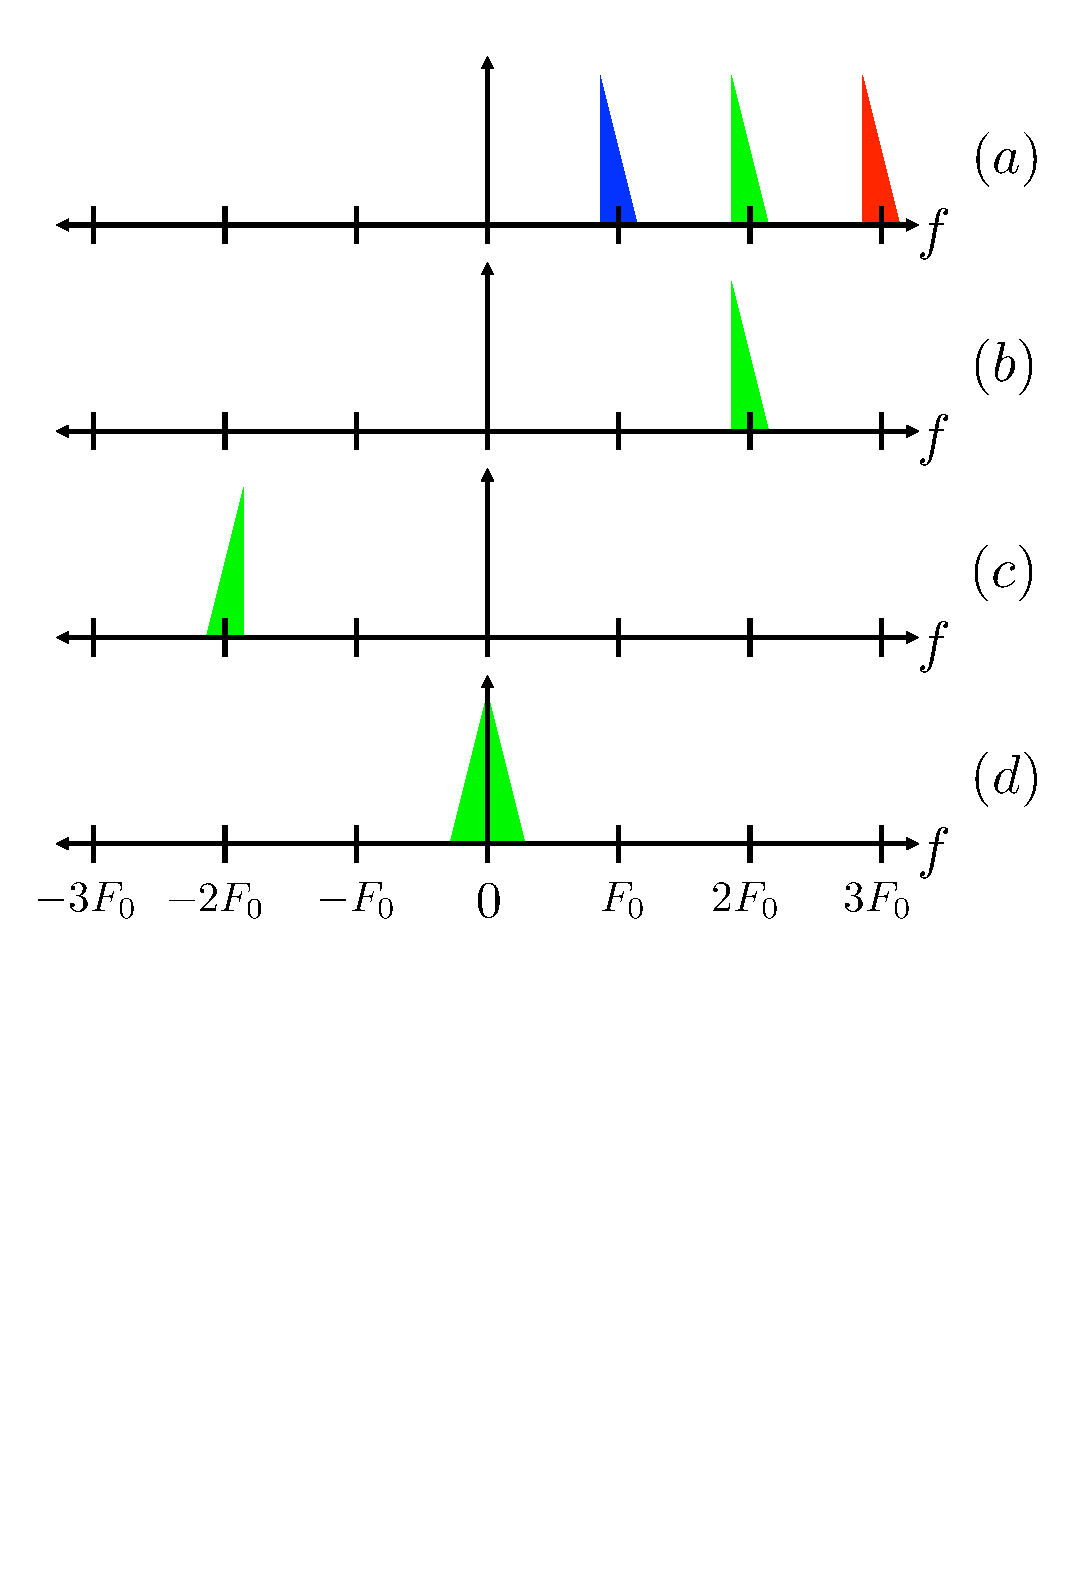
\includegraphics[width=.62\textwidth]{harmonic_envelope}
        \caption{Magnitude of spectrum for equations \ref{eq:harmonic_envelope_spectrum_a} - \ref{eq:harmonic_envelope_spectrum_d}}\label{fig:harmonic_envelope}
%        \caption{$(a) | \widehat{X}[n,f) |$
%    				$(b) | \widehat{X}_1[n,f) |$
%				$(c) | \widehat{X}_1^*[n,-f) |$
%				$(d) | \widehat{X}_1[n,f) * \widehat{X}_1^*[n,-f) |$}
\end{figure}

The envelope can always be acquired from the squared envelope by a final square root operation.  This operation introduces nonlinearities at multiples of $F_0$ that are difficult to analyze.  For mathematical convenience, during our analysis we can consider the squared envelope.  This final square root operation will remain constant across all examples which allows us to not consider it.

\begin{align}
\label{eq:square_root_relationship}
m_1[n] = \Big|\widehat{x}_1[n]\Big| = \Big[ \widehat{x}_1[n] \widehat{x}_1^*[n] \Big]^\frac{1}{2}
\end{align}

\subsection{Estimated Envelope}

Let's now evaluate our estimate, using equation~\ref{eq:envelope_extraction}.  As stated above, we consider the squared envelope.

\begin{align}
\tilde{m}_k^2[n] =& \Big| \widehat{x}[n]e^{-j \omega_kn} * h_k[n]]  \Big|^2 \nonumber \\
%
=& \Bigg|  \sum\limits_{l=0}^K m_l[n]e^{j(\theta_l[n] - \omega_k[n])}*h_k[n] \Bigg|^2 \nonumber \\
%
\approx& \Bigg|  \sum\limits_{l=0}^K m_l[n] \Big(e^{j(\theta_l[n] - \omega_k[n])}*h_k[n] \Big) \Bigg|^2 \nonumber \\
%
\label{eq:estimated_envelope_squared}
=& \Bigg|  \sum\limits_{l=0}^K m_l[n] e^{j\omega_{k,l}n} H_k\big(e^{j\omega_{k,l}}\big) \Bigg|^2 \\
%
\label{eq:downshift_radian_frequency}
\omega_{k,l} =& 2\pi\frac{(l+1)F_0 - F_{ds,k}}{F_s} \\
%
h_k[n] \Longleftrightarrow& H_k\big(e^{j\omega}\big)
\end{align}

$\omega_{k,l}$ is the downshifted center frequency of the $l$'th harmonic for the estimate of the $k$'th envelope.  $H_k\big(e^{j\omega}\big)$ is the discrete Fourier transform (DFT) of $h_k[n]$.

Expanding equation~\ref{eq:estimated_envelope_squared} we get:

\begin{align}
\tilde{m}_k^2[n] =& \sum\limits_{l=0}^K \sum\limits_{i=0}^K m_l[n] m_i^*[n] e^{j(l-i)F_0} H_k\big(e^{j\omega_{k,l}}\big)H_k^*\big(e^{j\omega_{k,i}}\big) \\
%
%
%
=& \sum\limits_{l=0}^K \Big|m_l[n]\Big|^2 \Big|H_k\big(e^{j\omega_{k,l}}\big)\Big|^2 \nonumber \\
%
%
+& e^{-j2\pi \frac{F_0}{Fs}n} \sum\limits_{l=0}^{K-1} m_l[n] m_{l+1}^*[n] H_k\big(e^{j\omega_{k,l}}\big)H_k^*\big(e^{j\omega_{k,l+1}}\big) \nonumber \\
%
+&  e^{j2\pi \frac{F_0}{Fs}n} \sum\limits_{l=1}^{K} m_l[n] m_{l-1}^*[n] H_k\big(e^{j\omega_{k,l}}\big)H_k^*\big(e^{j\omega_{k,l-1}}\big) \nonumber \\
%
%
+& e^{-j2\pi \frac{2F_0}{Fs}n} \sum\limits_{l=0}^{K-2} m_l[n] m_{l+2}^*[n] H_k\big(e^{j\omega_{k,l}}\big)H_k^*\big(e^{j\omega_{k,l+2}}\big) \nonumber \\
%
+& e^{j2\pi \frac{2F_0}{Fs}n}  \sum\limits_{l=2}^{K} m_l[n] m_{l-2}^*[n] H_k\big(e^{j\omega_{k,l}}\big)H_k^*\big(e^{j\omega_{k,l-2}}\big) \nonumber \\
%
%
+& ... \nonumber \\
%
%
+& e^{-j2\pi \frac{KF_0}{Fs}n} m_0[n] m_K^*[n] H_k\big(e^{j\omega_{k,0}}\big)H_k^*\big(e^{j\omega_{k,K}}\big) \nonumber \\
%
+& e^{j2\pi \frac{KF_0}{Fs}n}  m_K[n] m_0^*[n] H_k\big(e^{j\omega_{k,K}}\big)H_k^*\big(e^{j\omega_{k,0}}\big)
\end{align}

We can now think of $\tilde{m}_k[n]$ as a combination of terms each centered at $iF_0$ where the magnitude of each term is:

\begin{align}
\Big| \tilde{m}_{k,iF_0}[n] \Big| =& \Bigg[ \sum\limits_{l=0}^{K-|i|} \Big| m_l[n]\Big| \Big|m_{l+i}[n]\Big| \Big|H_k\big(e^{j\omega_{k,i}}\big)\Big| \Big|H_k\big(e^{j\omega_{k,l+i}}\big)\Big|\Bigg]^\frac{1}{2}, \quad -K \leq i \leq K
\end{align}

Evaluated at DC:

\begin{align}
\Big| \tilde{m}_{k,0F_0}[n] \Big| =& \Bigg[  \sum\limits_{l=0}^K \Big|m_l[n]\Big|^2 \Big|H_k\big(e^{j\omega_{k,l}}\big)\Big|^2 \Bigg]^\frac{1}{2}
\end{align}

\subsection{3 Harmonic Example: Estimated Envelope}

Let's go back to our three harmonic example.  We are again trying to acquire the 1st harmonic, $m_1[n]$ (green).  We define $\omega_1 = 2F_0$.

\begin{figure}[!ht]
  \centering
    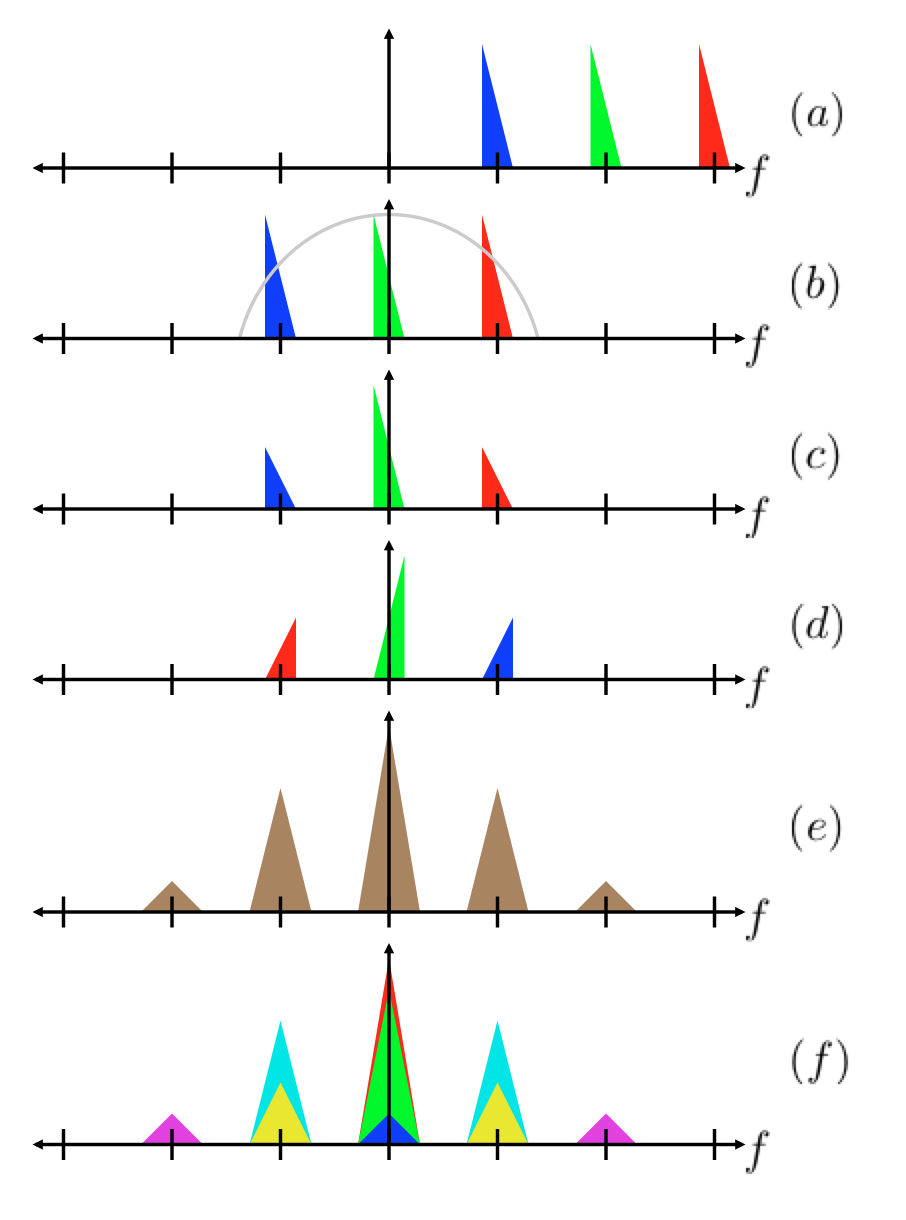
\includegraphics[width=.62\textwidth]{harmonic_envelope_estimate} 
    \caption{$(a) | \widehat{X}[n,f) |$   
    				$(b) | \widehat{X}[n,f - 2F_0) |$  
				$(c) | \widehat{X}[n,f - 2F_0) | | H_1(f) |$
				$(d) | \widehat{X}^*[n,-f + 2F_0) | | H_1(-f) |$
				$(e) | \mathcal{F} \{ \tilde{m}_1^2[n] \} |$
				$(f)$ contributions of separate components of $(e)$}\label{fig:harmonic_envelope_estimate}
\end{figure}

We can see the relationships

\begin{align}
\label{eq:harmonic_estimate_fig_a}
\widehat{x}[n] \Longleftrightarrow& \widehat{X}[n,f) \\
\widehat{x}[n]e^{-j2\pi \frac{2F_0}{F_s}n} \Longleftrightarrow& \widehat{X}[n,f - 2F_0) \\
\widehat{x}[n]e^{-j2\pi \frac{2F_0}{F_s}n} * h_2[n] \Longleftrightarrow& \widehat{X}[n,f - 2F_0) H_1(f) \\
\label{eq:harmonic_estimate_fig_e}
\tilde{m}_1^2[n] \Longleftrightarrow& \widehat{X}[n,f - 2F_0) H_1(f) * \widehat{X}^*[n,-f + 2F_0) H_1^*(-f)
\end{align}

Equations \ref{eq:harmonic_estimate_fig_a}  -\ref{eq:harmonic_estimate_fig_e} are visualized in figure~\ref{fig:harmonic_envelope_estimate}. The interesting part of figure~\ref{fig:harmonic_envelope_estimate} is $(f)$.  We see our green component that we were looking for, however there are a whole lot of other things that we didn't want.

Figure~\ref{fig:harmonic_envelope}$(d)$ is equivalent to the green component of  figure~\ref{fig:harmonic_envelope_estimate}$(f)$ if our filter $|H_1(f)| = 1$ when $f \approx 0$.

The other components come from interactions with the unwanted harmonics that we failed to completely filter out.  For clarity the convolution is visualized in figures \ref{fig:harmonic_envelope_2F0}, \ref{fig:harmonic_envelope_F0}, \ref{fig:harmonic_envelope_0}.  Positive and negative components are mirror images so the positive components are not explicitly visualized.

\begin{figure}[!ht]
   \centering
    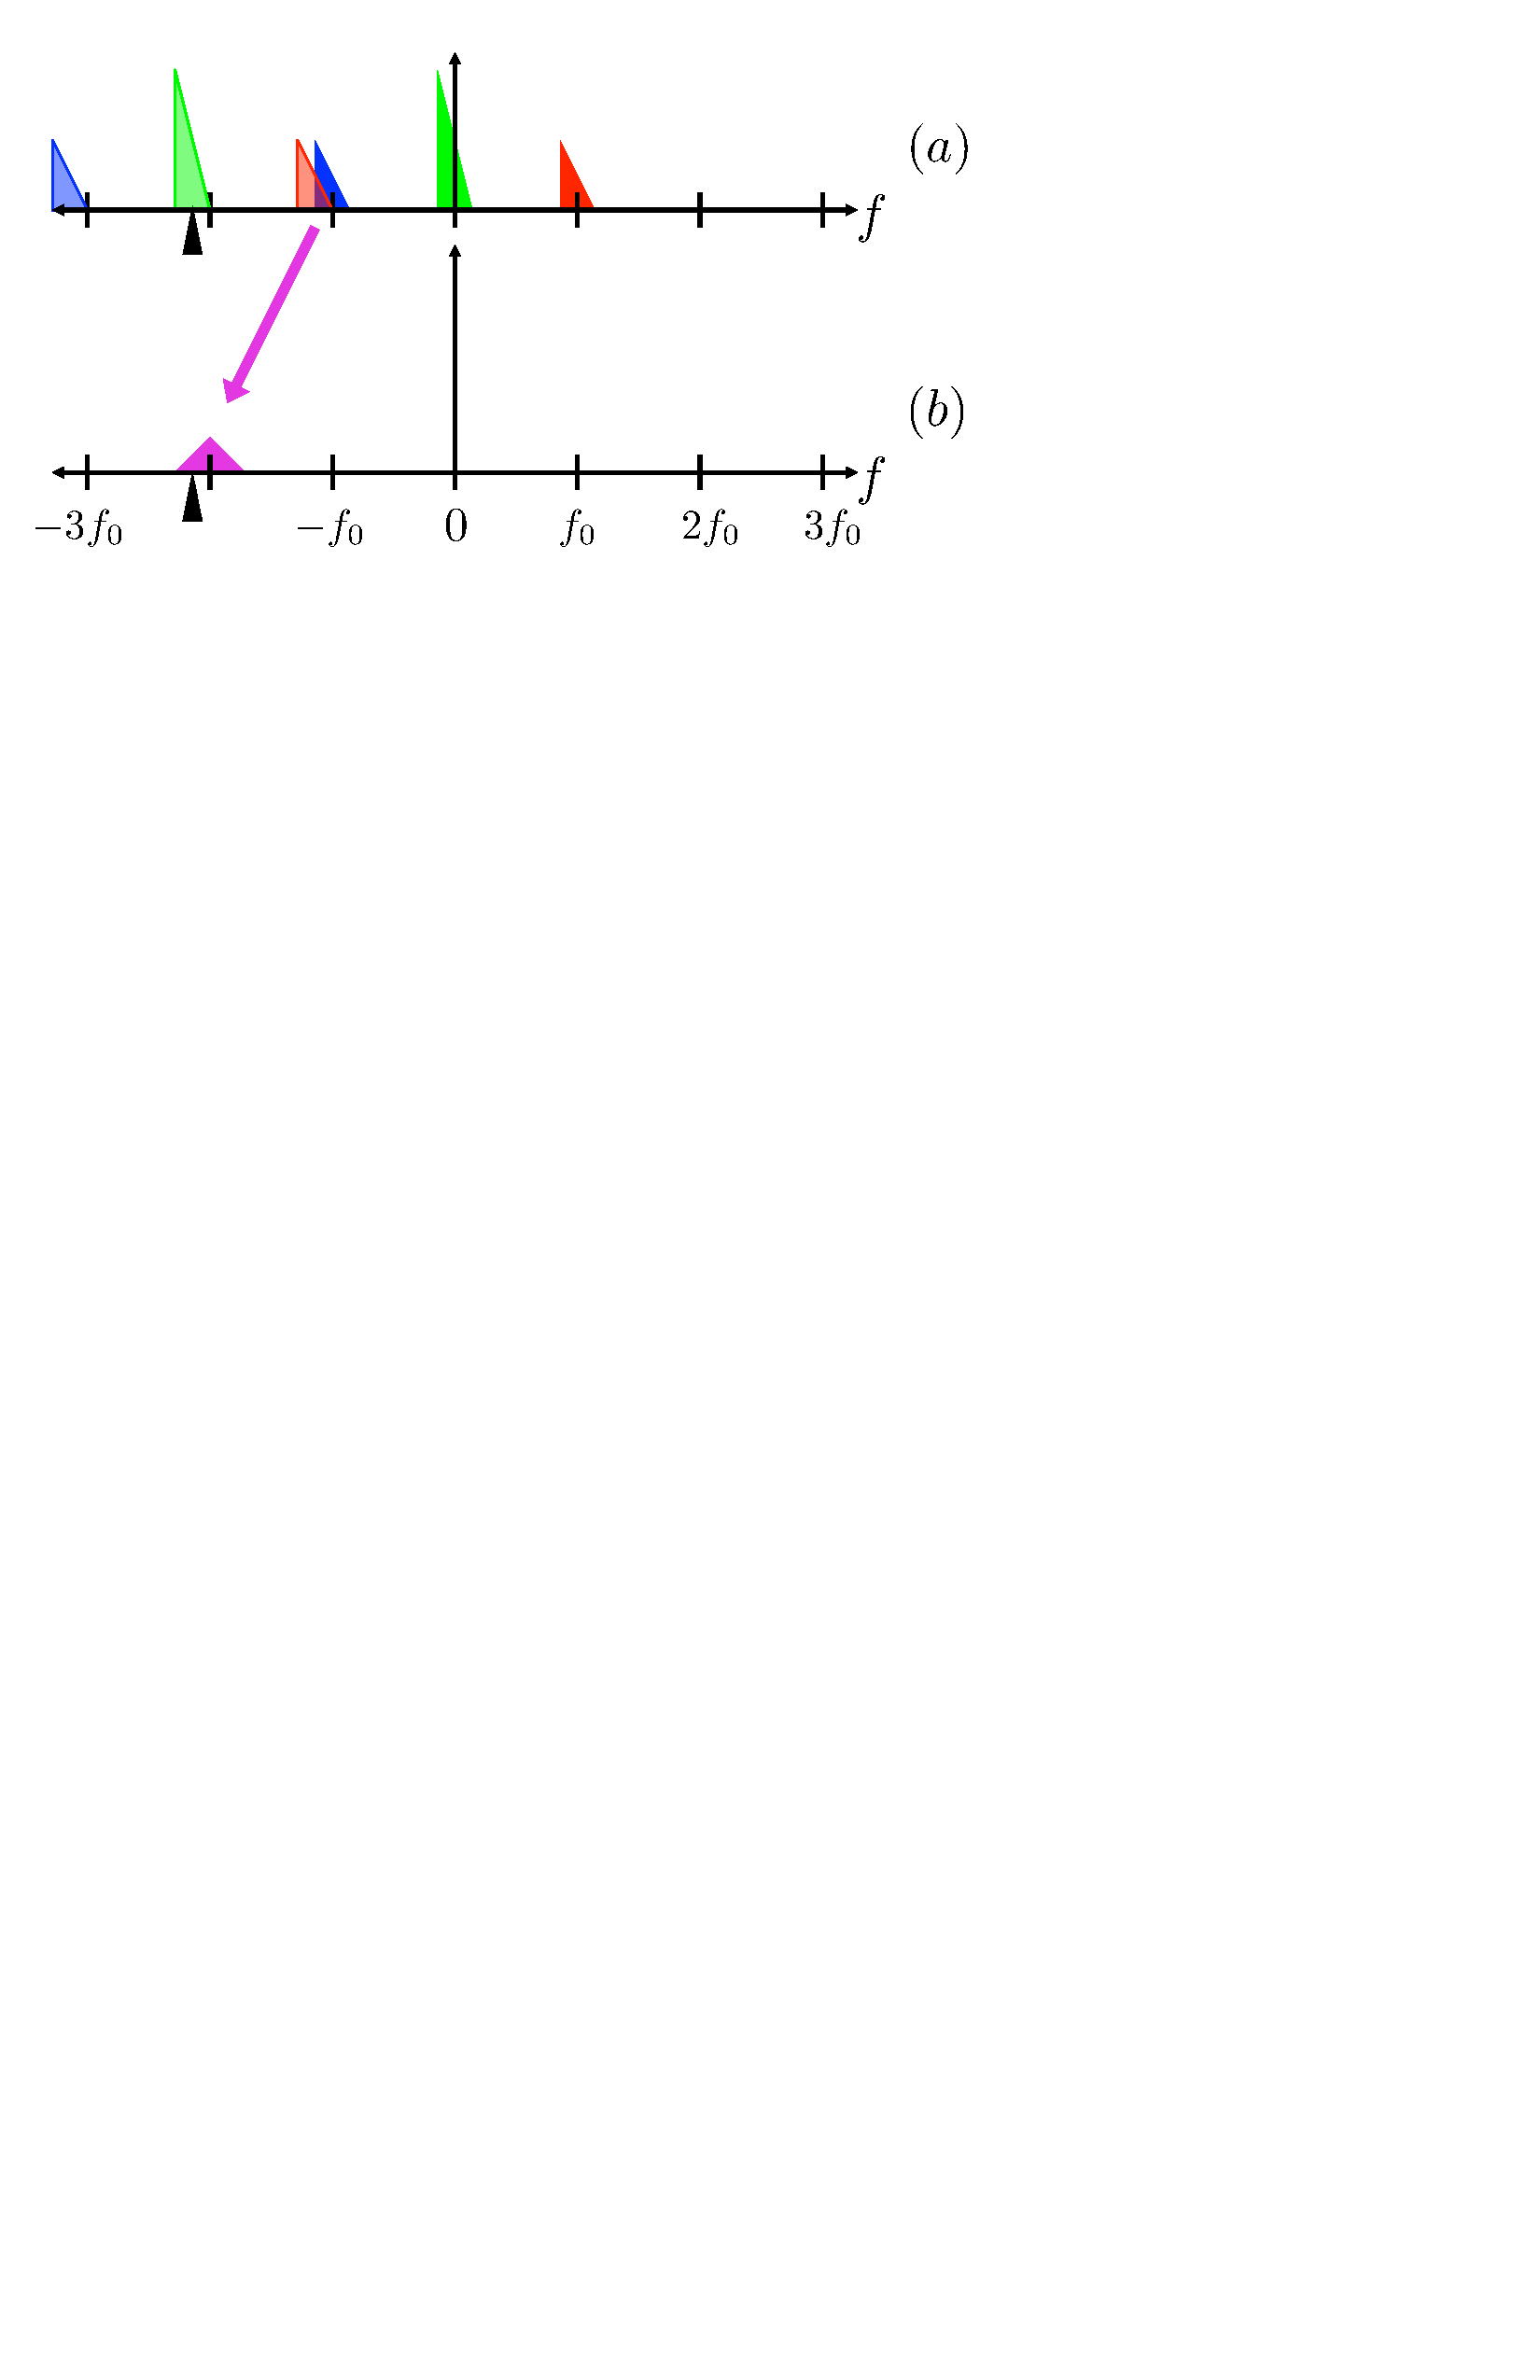
\includegraphics[width=.62\textwidth]{harmonic_envelope_2F0}   
    \caption{Envelope Estimate $-2F_0$ Component}\label{fig:harmonic_envelope_2F0}
    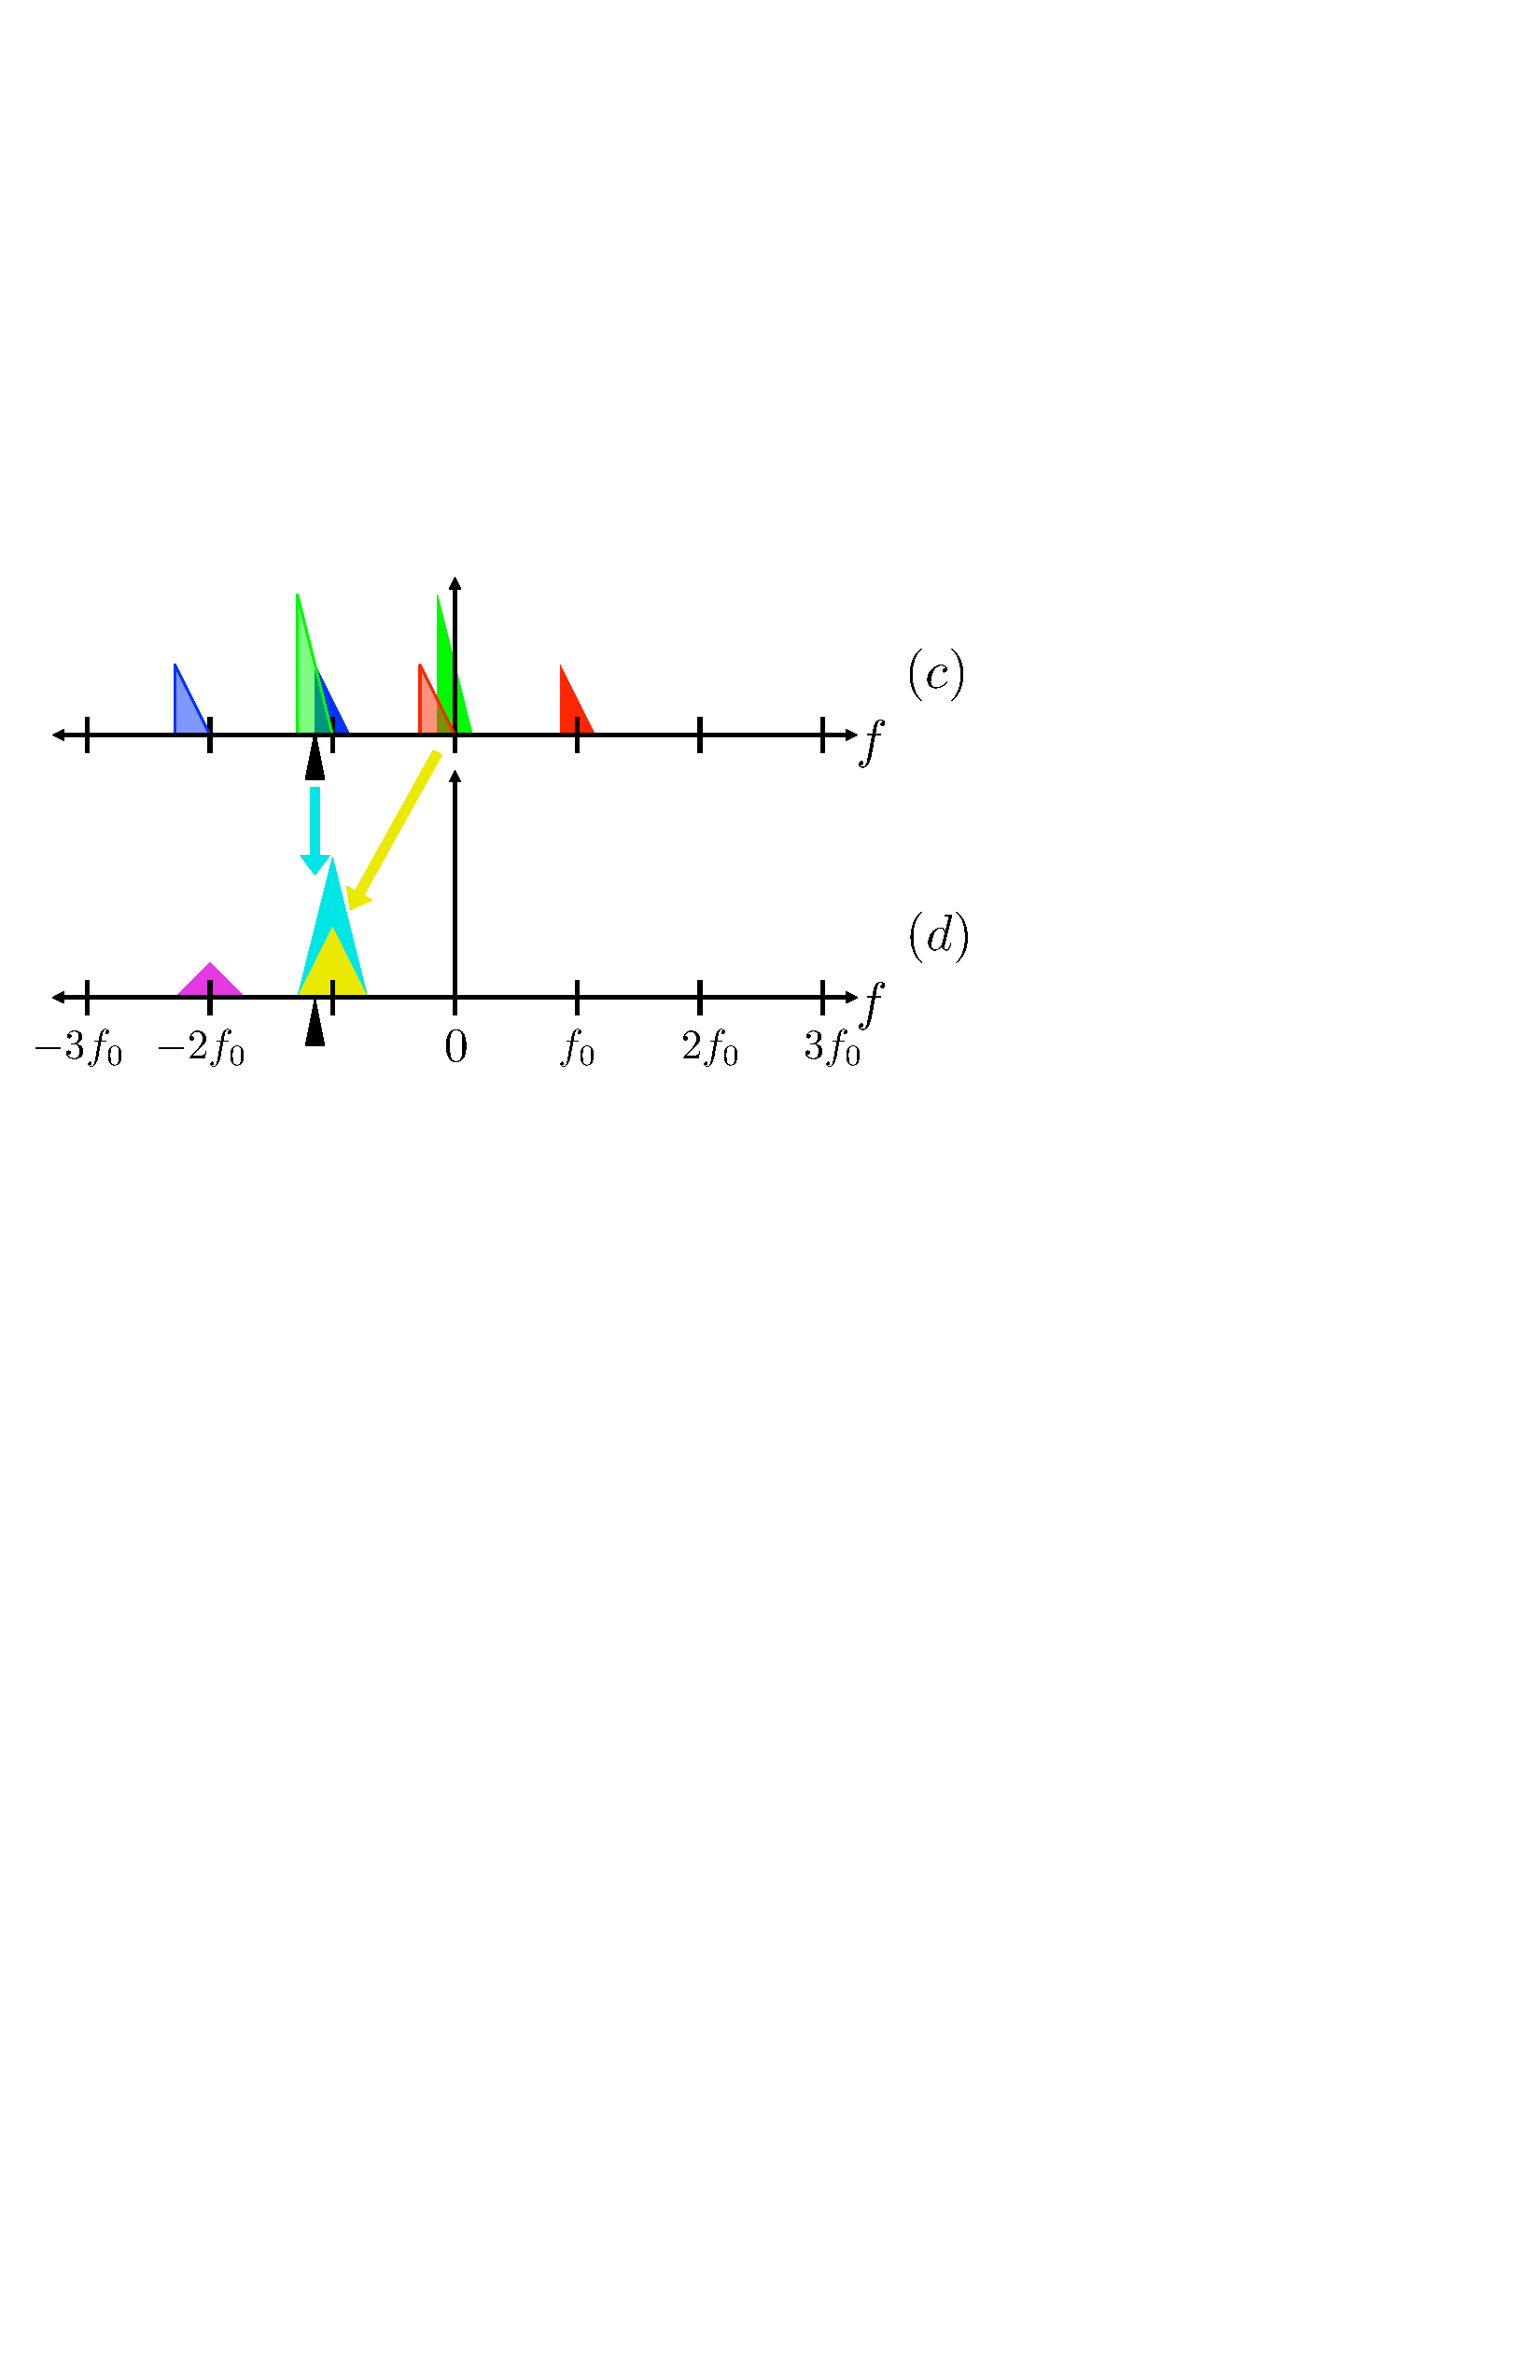
\includegraphics[width=.62\textwidth]{harmonic_envelope_F0} 
    \caption{Envelope Estimate $-F_0$ Component}\label{fig:harmonic_envelope_F0}
    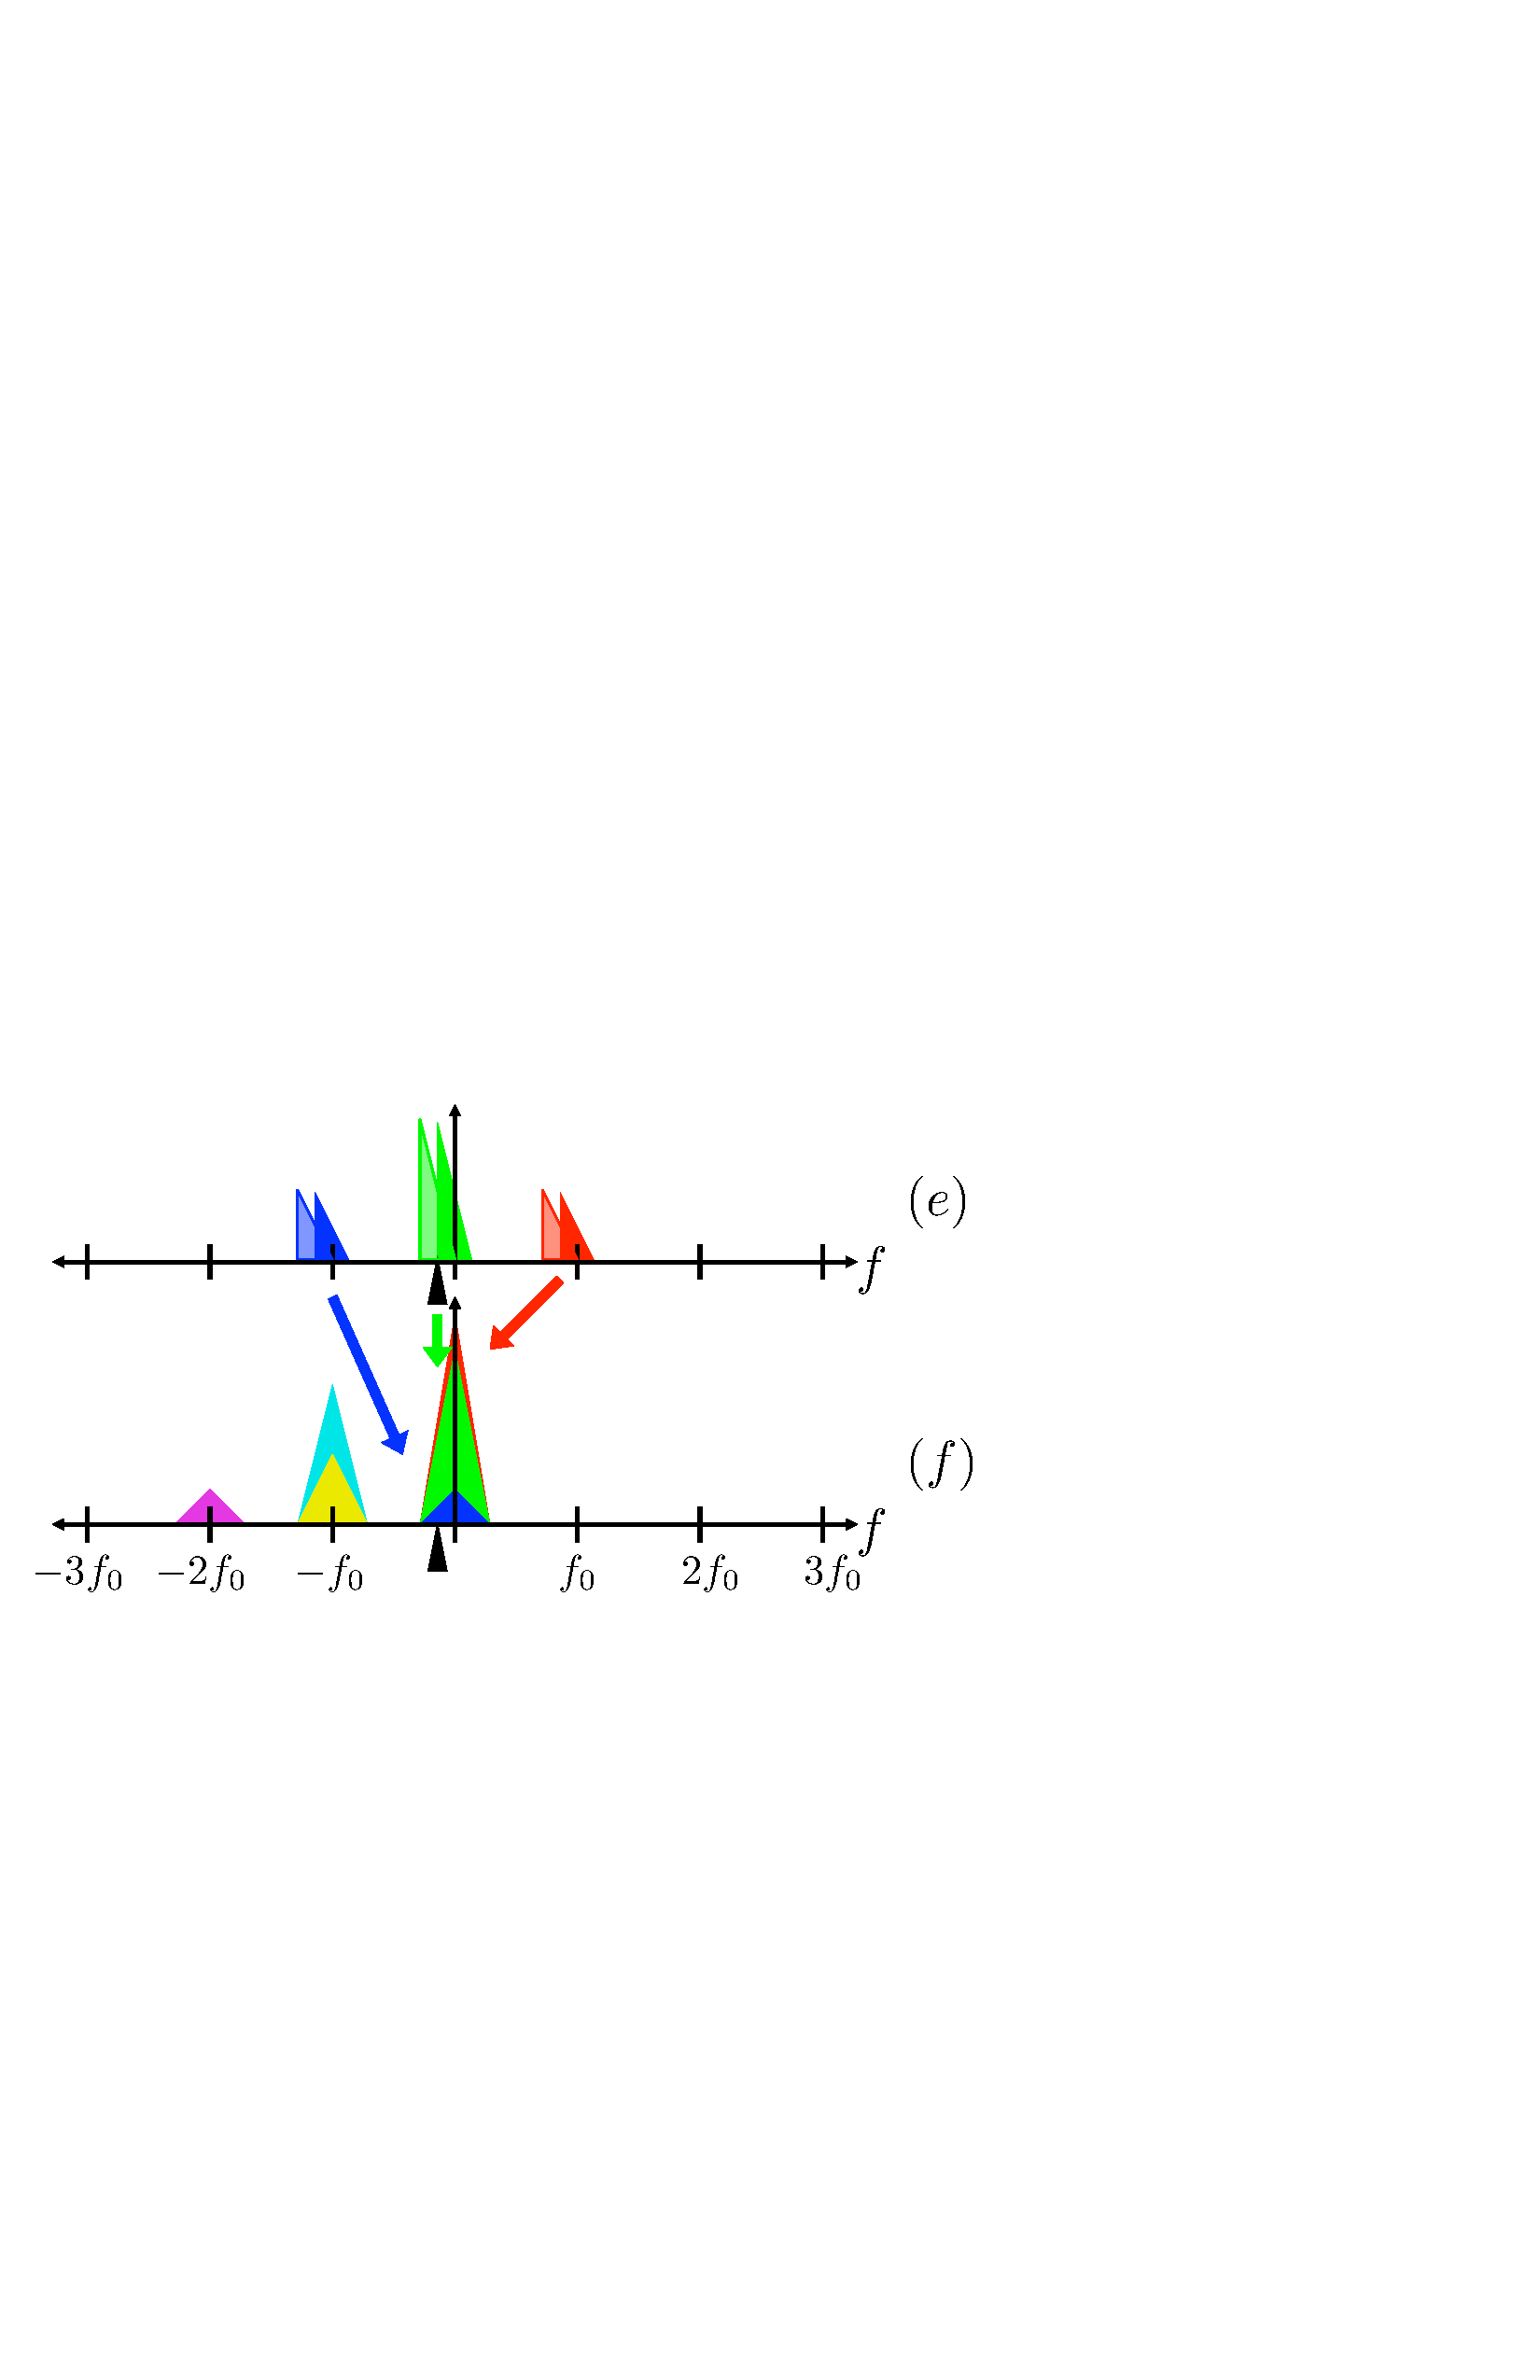
\includegraphics[width=.62\textwidth]{harmonic_envelope_0}
    \caption{Envelope Estimate Baseband Component}\label{fig:harmonic_envelope_0}
\end{figure}

\section{Steady-State Metrics}

In considering how well our envelope $\tilde{m}_k[n]$ estimates $m_k[n]$ there are three important metrics.  We will now discuss each in detail.

\subsection{Coherent Gain}

Coherent gain is defined as the gain of the harmonic of interest, $k$.

\begin{align}
G_k = \Big| H_k\big(e^{j\omega_{k,k}}\big) \Big|
\end{align}

Recalling equation~\ref{eq:downshift_radian_frequency}, if $F_{ds,k} = (k+1)F_0$ then, $w_{k,k} = 0$ and the coherent gain is simply the DC gain of the filter.

\begin{align}
G_k = \Big| H_k(0) \Big| = \sum_n h_k[n]
\end{align}

We may further simplify this by normalizing our filter such that $\Big| H_k(0) \Big| = 1$.  Of course, our downshift frequency won't be ideal in real systems.  Factors to consider include the quantization of $F_{ds,k}$ and the accuracy of $F_0$ estimation.

A similar metric, brought up in [REF] is termed scalloping loss, or picket-fence effect.  This is the effect of the harmonic falling in between filter centers.

\subsection{scalloping loss}

CONTINUEHERE1

[windows for harmonic analysis]

scalloping loss or picket-fence effect, ratio of coherent gain for tone located half a bin from DFT sample point to coherent gain for tone located exactly at sample point

\begin{align}
scalloping loss = \frac{| H(\frac{1}{2} \frac{F_s}{N}) |}{H(0)}
\end{align}

"althought scalloping loss is useful, it's not entirely informative.  if the scalloping loss if high, then this relates to a sharp cutoff which is actually good for increasing purity of the harmonic"

worst case processing loss = scalloping loss * PL
where PL is reduced gain of window (which i have been canceling out)
**where does worst case processing loss fit in?**

\subsection{Harmonic SIR}

Continuing our focus on the baseband, another question is: what is the contribution of the target harmonic versus the others?  The baseband component is contributed to by spectral leakage due to non-ideal filters.  This is visualized as the red and blue in figure~\ref{fig:harmonic_envelope_0}$(f)$.  The harmonic signal-to-interference-ratio (SIR) quantifies the ratio of target harmonic to spectral leakage.

\begin{align}
SIR_k =& \frac{\Big| H_k\big(e^{j\omega_{k,k}}\big) \Big|} {\Bigg[ \sum\limits_{l=0}^K \Big|H_k\big(e^{j\omega_{k,l}}\big)\Big|^2 \Bigg] ^ \frac{1}{2}}
\end{align}

The terms will roll off as the harmonic center frequencies get further away from $F_{ds,k}$, so typically $SIR_k$ is sufficiently described by only one or two harmonics on either side of the $k$'th, i.e. $k-2 \leq l \leq k+2$.

Harmonic SIR does not describe the true signal-dependent SIR, as varying envelope magnitudes across harmonics will change this, however it does provide an objective measure of the quality of our system to arbitrary harmonic inputs.

% one measure of spectral leakage is asymptotic falloff (db/octave) of sidelobes [windows for harmonic analysis]

\subsection{Modulation Depth}

Finally, we consider the magnitude of each bandpass component relative to baseband.  These terms appear in our envelope estimate as modulations at rates that are multiples of $F_0$.  Because of the forced symmetry of the real envelope we only need to consider positive frequencies, $iF_0$.

\begin{align}
D_{k,i} =& \frac{\Bigg[ \sum\limits_{l=0}^{K-i} \Big|H_k\big(e^{j\omega_{k,l}}\big)\Big| \Big|H_k\big(e^{j\omega_{k,l+i}}\big)\Big|\Bigg]^\frac{1}{2}}
{\Bigg[ \sum\limits_{l=0}^K \Big|H_k\big(e^{j\omega_{k,l}}\big)\Big|^2 \Bigg] ^ \frac{1}{2}}, \quad 1 \leq i \leq K
\end{align}

The largest value and, for that reason, most important value is $D_{k,1}$, the modulation depth at $F_0$.

\section{Explicit Temporal Modulation}

PUT THE F0MOD FIG VS ACE FIG IN HERE!!!!!!

So our three metrics are coherent gain, harmonic SIR and modulation depth.  We aim for a coherent gain of $G_k = 1$, maximum possible SIR and one would think minimum modulation depth.

Interestingly, some current CI processing strategies such as ACE intentionally allow for induced modulations from non-isolated harmonics.  This provides a temporal cue to the user which plays into pitch percept.

The alternative is to use narrow enough filter cutoffs to eliminate these modulations, and then explicitly modulate the signal.  In this option we need further processing such as a pitch estimator to determine the modulation rate.

In this document we argue that the latter, explicit modulation option is better.  The reasoning is best shown by a motivational example.

Let's consider a single note played by two different instruments: clarinet and saxophone.  In this example $F_0 = 261Hz$.  The clarinet is interesting in that it only has energy at odd harmonics.

We attempt to estimate the 3rd harmonic, $m_3[n]$.  We first downshift by $-3F_0$, then lowpass filter.  The spectrum of each signal at this stage is visualized in figure~\ref{fig:clarinetVSsax_F}.  The top panel shows the output of a sufficiently narrow filter where the 3rd harmonic is isolated.  The bottom panel shows a different filter design that intentionally allows the two adjacent harmonics to pass through.  Here we start to see the problem, that despite the wide bandwidth filter, there is (almost) no energy around $\pm F_0$ for the clarinet because of the harmonic structure.  (There is something present however it's down 30dB.)

\begin{figure}[!ht]
  \centering
    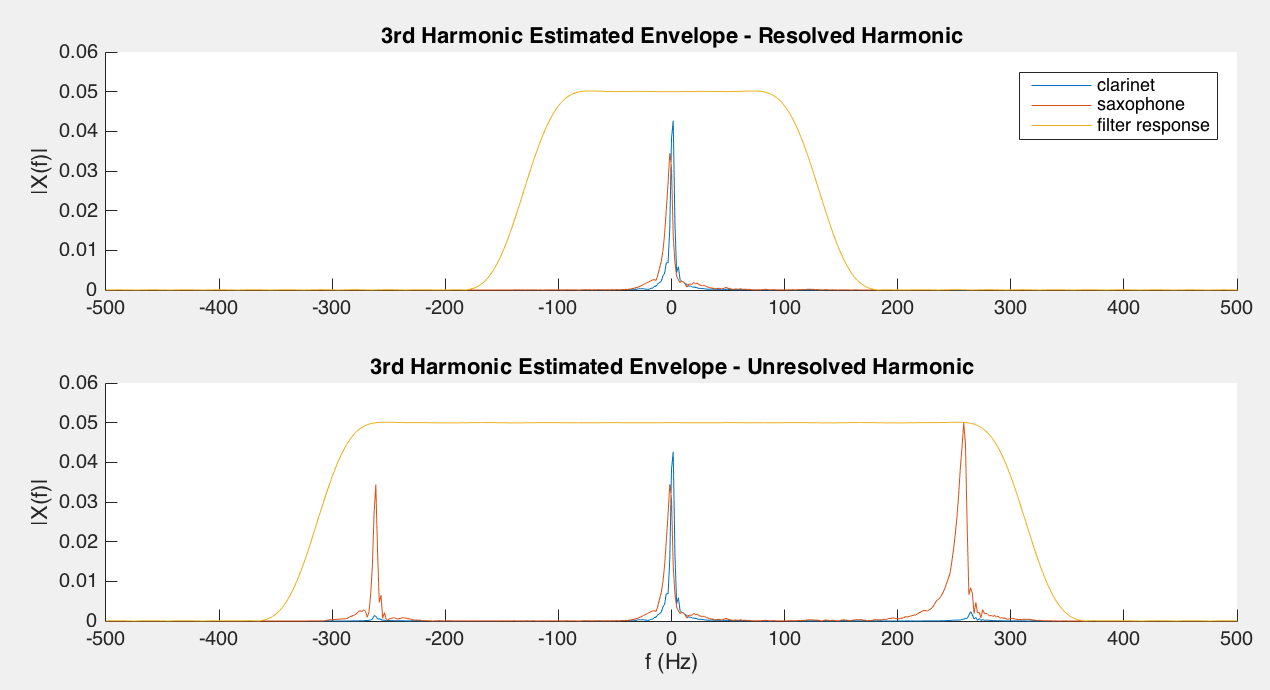
\includegraphics[width=1\textwidth]{clarinetVSsax_F}
    \caption{Clarinet vs Saxophone Harmonic Components}\label{fig:clarinetVSsax_F}
\end{figure}

Figure~\ref{fig:clarinetVSsax_T} shows the time-domain envelopes resulting from this processing.  The input signals were normalized such that the top panel shows the same signal power for both instruments.

The problem is clearly represented in the bottom panel, were we have a very large $F_0$ modulation in the saxophone envelope but little to no change in the clarinet.  The result is that we have a much stronger temporal pitch cue as well as louder overall volume to the saxophone.

\begin{figure}[!ht]
  \centering
    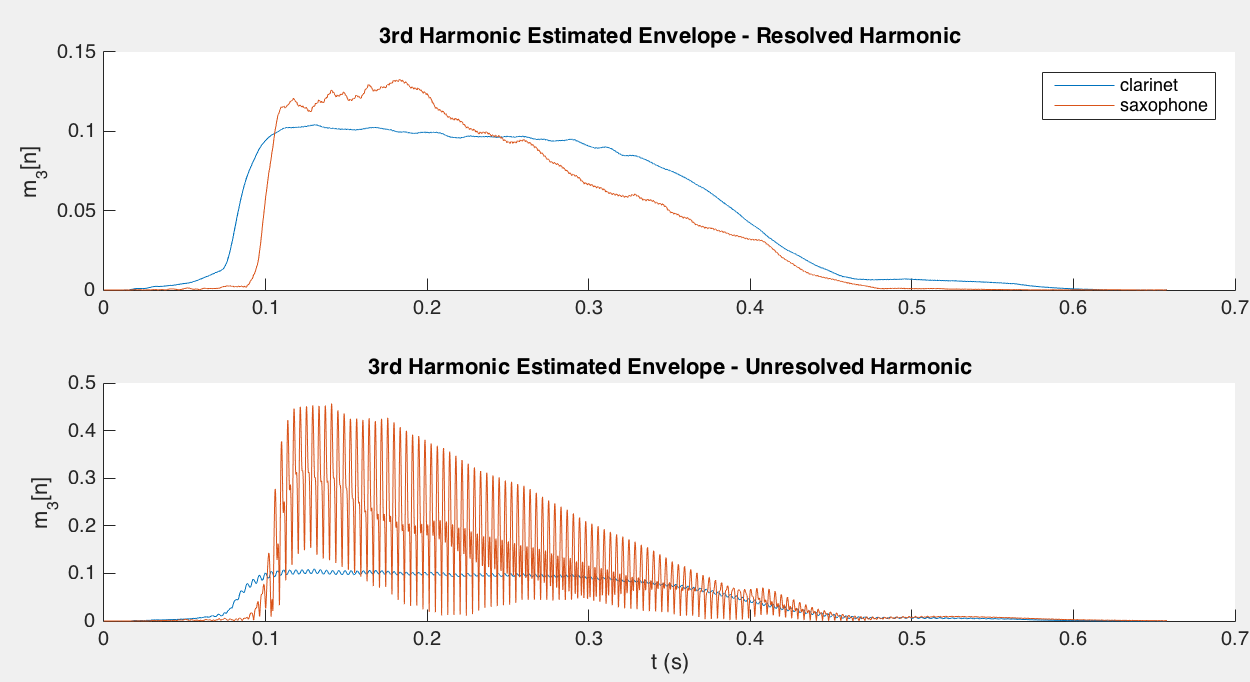
\includegraphics[width=1\textwidth]{clarinetVSsax_T}   
    \caption{Clarinet vs Saxophone Envelope Estimates}\label{fig:clarinetVSsax_T}
\end{figure}

Spectral leakage into other harmonic envelopes is not natural.  It forces the envelope to modulate as a function of the adjacent harmonics which, as we just saw, is signal dependent.  Furthermore, if we have uniform bandwidth filters, (as ACE does), the harmonic resolution will not behave as it does in the cochlea.

Beyond this example, explicit modulation decouples $F_0$ and modulation depth.  This way we have much more control over modulation depth while still making optimal design decisions for envelope extraction.  We can decide modulation depth as a function of how harmonic the signal is.  eTone [REF] uses a harmonic probability metric to do just that.

\subsection{Followup Filter}

Another thing to note is that regardless of downshift frequency, our harmonic envelope will always have it's energy centered at baseband and multiples of $F_0$.  An alternative way of eliminating induced modulations is to add a lowpass filter to the end of the processing chain.

There are a handful of research strategies [REF?] that have used this additional filter.  eTone's envelope follower is an example of this.

The main improvement to a followup filter is that we can guarantee to eliminate modulations.  This could also be achieved by designing a sufficiently narrow filter, $h_k[n]$ however this brings about a tradeoff, where the narrower our filter is the more susceptible we are to error in downshift frequency.

In terms of our three metrics, the followup filter will provide us with a robust coherent gain and guaranteed low modulation depth at the cost of lower harmonic SIR.

Another point to consider is the cost of adding an extra processing stage.  The additional stage means more memory, clock cycles and processing delay.

% Because of transient smearing, we will not be using this method

\section{Changing F0}

dips due to quantization

CONTINUEHERE2

maybe move the plot here?


\section{Transients}

``almostall of the hearingaidstestedhaveattack timeslessthan or equalto 10 ms. A little more than half of the hearingaidshad releasetimesof 50 ms or less.The rangeof the attack times varied from 1 to 23 ms'' [attack and release times of AGC hearing aids]

quantify for best case and worst case where worst case is the fastest transient relevant to music (this should also hinge on CI limitations)

maximum onset dynamic range "90ms - 10ms = 80ms"
and ratio of filter smeared range to max range
rinse and repeat for CI's

\section{Steady-State Evaluation of Strategies}

chosen parameter values to compare:
order 128, 256, 512
quantize 1, 31, 62, 125
cutoff, rectangular, hanning, adaptive butterworth

\subsection{Design Parameters}

As stated above the design can be summarized by downshift frequency and lowpass filter.

For our steady-state scenario the the ideal downshift frequency is simply $(k+1)F_0$.  The question is what degree of quantization is sufficient to estimate our signal.

For filter design we need to consider bandwidth as a function of filter order and filter/window type.  Ideally our cutoff is somewhere below $F_0$ but high enough to incorporate the narrow bandwidth of $m_k[n]$.

The filters can be different as a function of $k$.  This is a natural path to pursue if we consider the critical bands of the cochlea.  This will be discussed in more detail later in this document however for now we will assume $h_k[n] = h[n]$.  This is natural for harmonic envelopes as harmonics are linearly spaced.

\subsection{Coherent Gain}

Not overly interesting, just talk about scalloping loss and mention that number of dips is proportional to harmonic index k.

The interesting part here is the relationship between harmonics.  Where the fundamental will be at a minimum, the 1st harmonic is at a maxima, example:

$F_q = 125$

$F_0 = 182.5 = 1.5 F_q$ (right in between bins)

$2F_0 = 375 = 3 F_q$ (right on a bin)

<CONTINUE HERE>

[windows for harmonic analysis]

scalloping loss or picket-fence effect, ratio of coherent gain for tone located half a bin from DFT sample point to coherent gain for tone located exactly at sample point

\begin{align}
scalloping loss = \frac{| H(\frac{1}{2} \frac{F_s}{N}) |}{H(0)}
\end{align}

"althought scalloping loss is useful, it's not entirely informative.  if the scalloping loss if high, then this relates to a sharp cutoff which is actually good for increasing purity of the harmonic"

worst case processing loss = scalloping loss * PL
where PL is reduced gain of window (which i have been canceling out)
**where does worst case processing loss fit in?**

\subsection{Harmonic SIR}

Just note that major difference in filter order

\subsection{Modulation Depth}

Again...filter order

BW = F0/2
downshift = exp(kF0)

downshift quantization, bandwidth as function of F, F0?

modulation depth (kind of another SIR) as a function of downshift quantization and filter

\subsection{figures}

\section{ALL METRICS}

ENBW (accumulated noise)
PL (gain at DC)
PG (same as PL?)
scalloping loss (downshift quantization worst case)
worst case PL = PL*SL

harmonic SIR
harmonic gain (maybe not overly relevant due to AGC, etc)
					(how is it affected in a relative sense? worst vs best)
modulation depth (spectral leakage)
transients
changing F0 (scalloping loss dip only, and harmonic SIR)

\subsection{Harmonic Bandwidth}

what is it?  look at some waveforms and read some stuff.  maybe do this at the same time as transient times of instruments

\section{Adaptive Filters}

consider all metrics for adaptive filters, order 128, 256, 512


\chapter{Implementation Considerations}

\section{Efficient Interpolation Algorithm}

FFT with changeable window, and interpolate

Can this be done with different filter as function of F0?
We probably need to design the filters such that they pass reconstruction requirements

Is the actual equation just a sinc function times a phase shift?!

READ THIS: [An Intelligent FFT-Analyzer with Harmonic Interference Effect Correction and Uncertainty Evaluation]

\section{Mapping and Selection}

\chapter{-----------------------------------}


\chapter{Background}

\section{Acoustic Hearing}

Before discussing how cochlear implants are able to restore hearing in people with profound hearing impairment, it is useful to talk about how acoustic hearing works in normal listeners.

\subsection{Anatomy of the Ear}

tonotopic, critical bands, ...

\subsection{speech}

\subsection{pitch}

``frequencies in the range of 80-300 Hz encompassing F0 for nearly all adult males and many females and children.''
% [pitch_ranking_strategy_compare]

\subsection{other characteristics of sound}

\subsection{types of audio}
speech, music, harmonic, inharmonic, voiced, unvoiced
tonal, non-tonal, consonant disonant..., transient, steady state


\section{cochlear implants}
CI basics (CIS)
vague envelope concepts without math

mention CIS FWR = ABS()!!!

"In spite of the fact that this analog signal itself preserves most of the original temporospectral in- formation, the signal transfers to the auditory nerve is handicapped by the limited maximal firing fre- quency of the auditory nerve in response to the electrical stimulation. High synchronization of nerve fibers and the neural refractory period only allow for frequency transmission up to 1 kHz via tempo- ral coding alone. For frequencies above 1 kHz, the spectral information cannot be sufficiently trans- ferred by temporal coding alone. Multichannel im- plants have been developed to make use of the tonotopic organization in the cochlea and thus transmit more spectral information to the auditory nerve." \cite{somek2006coding}


"The HiRes120 strategy, used in the Advanced Bionics implant, is the first commercial stimulating strategy that uses the virtual channel technique. Virtual channels are created by adjusting the current level ratio of two neighboring electrodes."

channel mapping
    why only 8 at a time?
    ACE vs CIS and benefits of each
    
    
    
    ACE uses place cues as the primary source of encoding a sound's characteristics.  To this day it is still unclear as to what implications this has.  This is due to a combination of factors including the subjective nature of pitch and absence of a ground truth baseline in many CI users.  For example, high-pass filtering a sound may cause it to sound brighter.  In contrast low-pass filtering would cause a warm quality.  As stimulus change electrodes a CI user could claim to experience changes in the high-low quality of pitch when really they are experiencing changes in the bright-warm quality of spectral distribution, or more likely an ambiguous combination of both.

``Previous research had suggested that cochlear implant place pitch was more akin to brightness (an aspect of timbre) than to pitch. However, the Modified Melodies results supported the hypothesis that place pitch can support melody perception.'' [swanson thesis]

There is general consensus that place cues are not sufficient for encoding pitch.  Alternatively, temporal cues encoded as time-domain carrier modulations have shown to be promising.


``wideband vs feature extraction'' [F0F2-F0F1F2]
not sure what wideband implies, alternatively use temporal envelope cues.

``Another school of thought was based on speech production and perception, in which spec- tral peaks or formants, which reflect the reso- nance properties of the vocal tract, are extracted and delivered to different electrodes according to the presumed tonotopic relationship between the place of the electrode and its evoked pitch.'' %[trends_in_CIs]
F0F2, F0F1F2, MPEAK

    what is important?
        hearing for any general reason...safety, functionality
        speech recognition
    what is important and lacking?
        music appreciation
        tonal language
        SiN
        quality

\subsection{modulation depth}

``Previous CI psychophysical studies investigat- ing the pitch of sinusoidal amplitude-modulated pulse trains have shown considerable variation between subjects in terms of the modulation depths required for reliable discrimination of pitch (McKay et al., 1995; Geurts and Wouters, 2001). On average, modulation depths ranging from 10\% to 40\% of the electrical dynamic range were required, although some subjects required depths of almost 100\%. Converting these values to the acoustic dynamic range coded by the sound processor, which for the Nucleus 24 system is typically 30 dB, indicates that modulation depths in the acoustic signal of approximately 3 to 12 dB are required on average.'' %[pitch_ranking_strategy_compare]

\section{temporal fine structure}

explicit encoding vs ACE

clarinet example


% ========== Chapter 3

\chapter{Harmonic Envelopes}


\section{Envelope Extraction Methods}

``In most existing clinical sound processors, fine structure in the input acoustic signal is discarded, and only envelope information is preserved. ''  %[pitch_ranking_strategy_compare]


A classic way of analyzing audio signals is the sum-of-products model.  In this model a signal is represented as a sum of narrowband signals $x_k[n]$ at distributed center frequencies.  Each of the narrowband components is modeled as a product of a slow-time-varying envelope $m_k[n]$ and a fast-time-varying carrier $c_k[n]$.

%$$x[n] = \sum\limits_k x_k[n] = Re\bigg\{ \sum\limits_k m_k[n] c_k[n] \bigg\}$$

\begin{equation}
\label{eq:sum-of-products}
x[n] = \sum\limits_k x_k[n] = \sum\limits_k m_k[n] c_k[n]
\end{equation}


We are assuming here that $x[n]$ is a strictly real-valued signal.

This model works especially well for harmonic signals, where each individual harmonic is represented by a narrowband component.  In the case of speech, one could think of the collection of carriers as the harmonic signal generated by the vocal tract, while the modulators together represent the resonant structure that distinguishes separate vowels. <--figure?!  Continue...

In this model information such as gender of talker, intonation or musical pitch would be dominantly characterized by the carriers.  The resonant information that distinguishes different vowels or the unique formant structure of a particular instrument would be encoded in the modulators.

The sum-of-products model is particularly convenient for CIs for a few different reasons. For starters, this model is naturally similar to the way our ears work. "mechanical fourier transform" [chimeara] The initial goal of CI researchers was to achieve speech recognition.  Given the limitations of CIs, encoding only the modulation information acts as a form of lossy data compression.

More reasons this model is good, musically?
Why is it good for CIs?

Provided the above motivation for sum-of-products signal modeling we come to the challenge of how exactly to decompose a signal.  There are many different ways of doing this but they broadly fall into one of two categories: incoherent methods and coherent methods.

\begin{figure}[!ht]
  \centering
    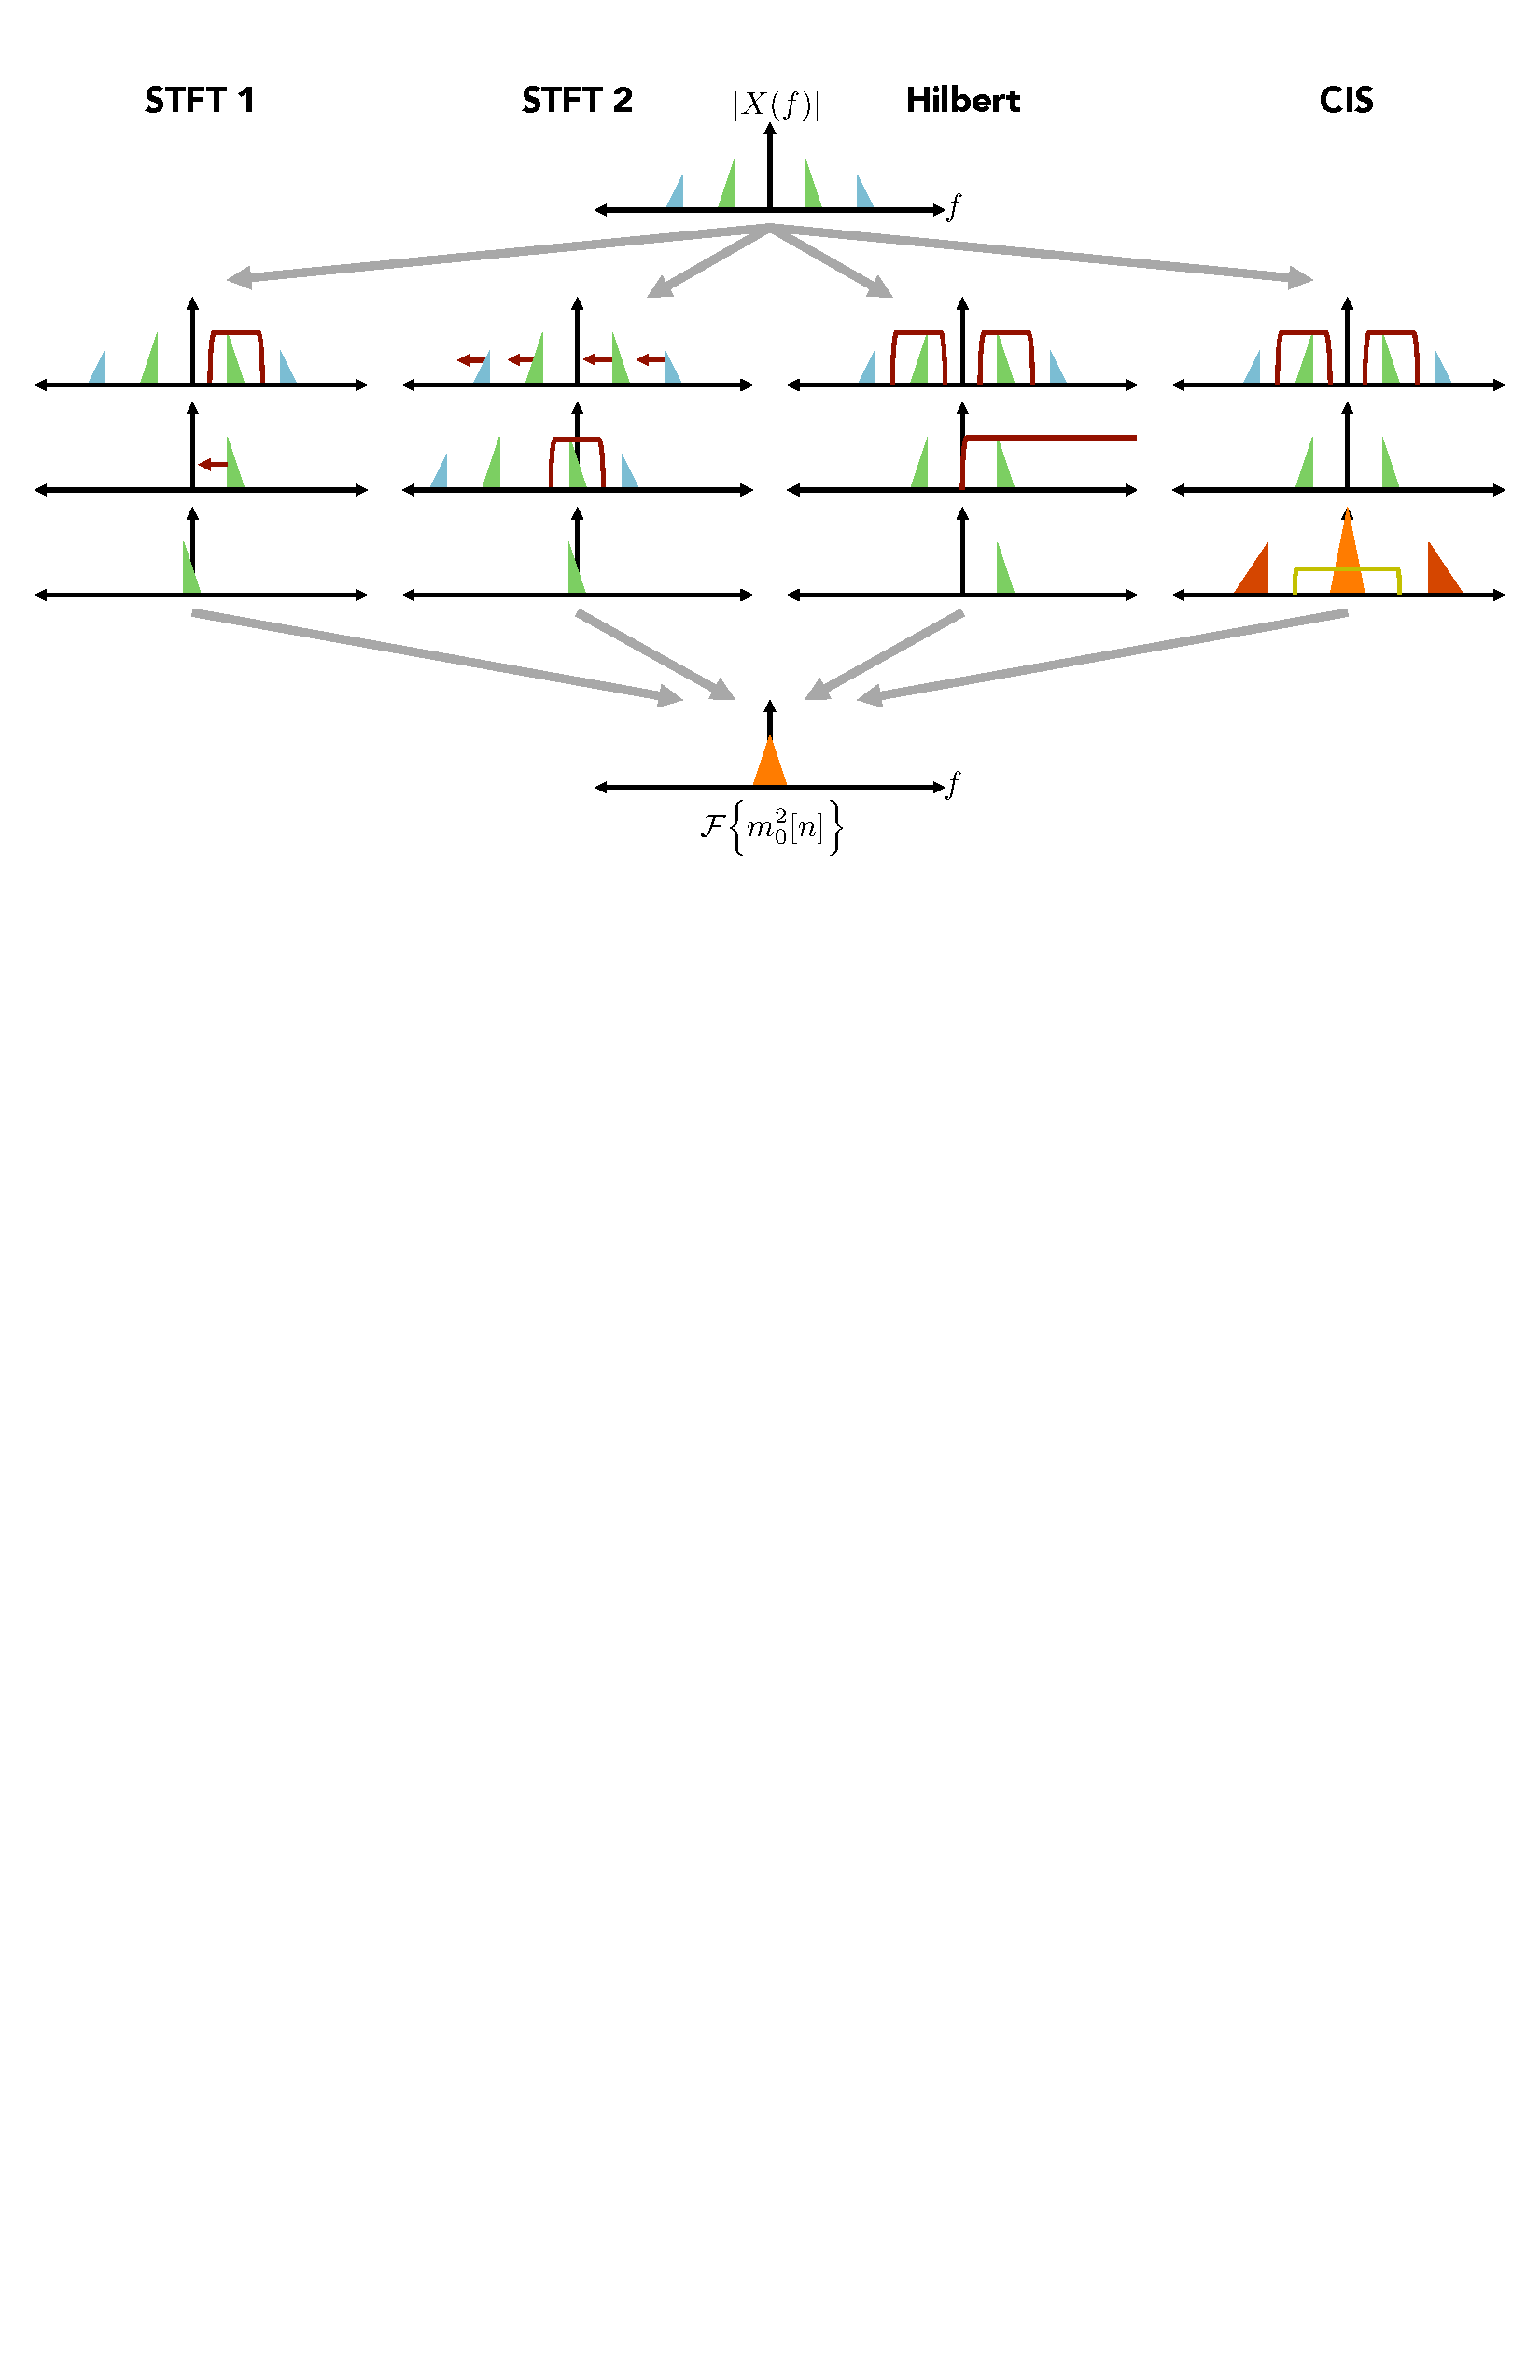
\includegraphics[width=1.0\textwidth]{STFTvsHILBERTvsCIS}   
    \caption{STFT vs Hilbert vs CIS}
\end{figure}

\subsection{Incoherent Methods - Short Time Fourier Transform (STFT)}

With incoherent methods, an envelope is extracted independent of the carrier; no information about the carrier is taken into account prior to envelope extraction.

One such method is the short-time Fourier transform (STFT), which has two classic interpretations: a series of windowed Fourier transforms (each at a different time instant) or a collection of uniform bandpass filters (each at a different center frequency).  For our purposes we will be using the later.

An STFT bin at discrete time $n$ and discrete frequency $k$ is defined as:

\begin{align}
\label{eq:STFTdefinition}
X[n,k] = \sum\limits_{r=-\infty}^{\infty} x[r] w[r - n] e^{-j\frac{2\pi}{N}kr}, \qquad 0 \leq k < N
\end{align}

Defining a new variable $r' = r - n$ and defining our window such that  $w[n] = 0$ for $n < 0$ or $N \leq n$,

\begin{align}
X[n,k] =& \sum\limits_{r'=0}^{N-1} x[n + r'] w[r'] e^{-j\frac{2\pi}{N}k(n + r')} \nonumber \\
=& e^{-j\frac{2\pi}{N}kn} \sum\limits_{r'=0}^{N-1} x[n + r'] w[r'] e^{-j\frac{2\pi}{N}kr'}
\end{align}

Let $X[n,k]$ be represented in polar form as the following

\begin{equation}
X[n,k] = \vert X[n,k]\vert e^{j\angle X[n,k]}
\end{equation}

If we assume that the window $w[n] \neq 0$ for $0 \leq n \leq N-1$ then we have the inverse

\begin{align}
x[n + r'] =& \frac{1}{Nw[r']}  \sum\limits_{k=0}^{N-1} X[n,k] e^{j\frac{2\pi}{N}k(n+r')} \nonumber \\
=& \frac{1}{Nw[r']}  \sum\limits_{k=0}^{N-1} \vert X[n,k]\vert e^{j(\frac{2\pi}{N}k(n+r') + \angle X[n,k])} \\
x[n] =&\sum\limits_{k=0}^{N-1}  \frac{1}{Nw[0]}  \vert X[n,k]\vert e^{j(\frac{2\pi}{N}kn + \angle X[n,k])}
\end{align}

Without loss of generality we can use a STFT hop-factor of one sample.  In the case of a greater hop factor we would need to compute $x[n]$ from (2.5) [FILL IN THIS REF] for some samples.  Of course, if the hop factor is greater than $N$ we cannot fully reconstruct the signal.  (This is why we will recurringly see $w[0]$)

We can now clearly see our sum-of-products model

\begin{align}
\label{eq:envelope_STFT}
m_{k,STFT}[n] =  \frac{1}{Nw[0]}  \vert X[n,k]\vert \\
c_{k,STFT}[n] = e^{j(\frac{2\pi}{N}kn + \angle X[n,k])}
\end{align}

We can think of the STFT as a series of $N$ LTI systems that each downshift the input signal, then lowpass filter.  This can be seen mathematically if we rewrite equation \ref{eq:STFTdefinition} as

\begin{align}
\label{eq:STFTasFilter}
X[n,k] =& \sum\limits_{r=-\infty}^{\infty} x[r] e^{-j\frac{2\pi}{N}kr} w[-(n - r)] \nonumber \\
=& x[n] e^{-j\frac{2\pi}{N}kn} * w[-n]
\end{align}

Then looking at our $N$ envelope-carrier pairs we see that the reconstruction of $x[n]$ will be real because with the exception of $k = 0$ and $k = \frac{N}{2}$ which correspond to a lowpass filter and highpass filter, the rest come in complementary pairs.

\begin{align}
pv \ \frac{2\pi (N-k)}{N} = \frac{-2\pi k}{N}, \qquad 0 < k < \frac{N}{2}
\end{align}

where $pv$ denotes principal value.  This directly relates to the property that for any real-valued $x[n]$,

\begin{align}
X[n,k] = X^*[n,N-k], \qquad 0 < k < \frac{N}{2}
\end{align}

FIG - reconstruction of STFT envelopes

\subsection{Incoherent Methods - Hilbert Transform}

Alternatively, a Hilbert transform uses the analytic signal to separate envelope from carrier.  We first acquire the bandpass signal

\begin{align}
x_k[n] = x[n] * h_k[n]
\end{align}

Where $h_k$ is a bandpass filter and $k$ has arbitrary limits.  Then using the analytic signal

\begin{align}
\widehat{x}_k[n] =& x_k[n] + jH\{x_k[n]\} \\
\label{eq:hilbert_envelope}
m_{k,hilbert}[n] =& \vert\widehat{x}_k[n]\vert \\
c_{k,hilbert}[n] =& cos(\angle\widehat{x}_k[n])
\end{align}

For it to remain true that $x[n]$ may be reconstructed from our decomposition $h_k[n]$ must be constrained such that 

\begin{align}
\sum_k h_k[n] = \delta[n]
\end{align}

It is important to note that unlike the STFT case, $c_{k,hilbert}[n]$ is real.  This is due to the conversion to an analytic signal (?.?) which eliminates negative frequencies.  [This is confusing, explain better, talk about reconstruction and maybe show figures showing how STFT is asymmetric and Hilbert is symmetric]

FIG - reconstruction of hilbert envelopes

Let us now compare this method to the STFT method.  Since "the Hilbert transform of a convolution is the convolution of the Hilbert transform on either factor" [wikipedia] we have 

\begin{align}
\label{eq:x_analytic}
\widehat{x}_k[n] =& x_k[n] + jH\{x_k[n]\} \nonumber \\
=& x[n] * h_k[n] + jH\{x[n] * h_k[n]\} \nonumber \\
=& x[n] * h_k[n] + x[n] * jH\{h_k[n]\} \nonumber \\
=& x[n] * [h_k[n]+  jH\{h_k[n]\}]
\end{align}

Now let us define our filter specifically as

\begin{align}
\label{eq:hilbert_constrained_filter}
h_k[n] = \frac{1}{Nw[0]}w[-n]cos(\frac{2\pi}{N}kn)
\end{align}

If we assume the sidelobes of $w[n]$ roll-off sufficiently fast in relation to the center-frequency $\frac{2\pi k}{N}$, we may approximate

\begin{align}
\mathcal{H}\{h_i[n]\} \approx& \frac{1}{Nw[0]}w[-n] H\{cos(\frac{2\pi}{N}in)\} \nonumber \\
=& \frac{1}{Nw[0]}w[-n]sin(\frac{2\pi}{N}in)
\end{align}

To verify the previous equation, consider the extremes:

1) $w[n] = 1$

2) $w[n] = \delta[n]$

TODO: verify this approximation claim

Plugging our filter \ref{eq:hilbert_constrained_filter} into \ref{eq:x_analytic}

\begin{align}
\widehat{x}_k[n] \approx& x[n] * \frac{1}{Nw[0]}w[-n]e^{j\frac{2\pi}{N}in} \nonumber \\
=& \frac{1}{Nw[0]}\sum\limits_{r=-\infty}^{\infty}x[n - r] w[-r] e^{j\frac{2\pi}{N}ir} \nonumber \\
\textrm{Let} \quad r' = -r \nonumber \\
=& \frac{1}{Nw[0]}\sum\limits_{r'=0}^{N-1} x[n + r'] w[r'] e^{-j\frac{2\pi}{N}kr'} \nonumber \\
=& \frac{1}{Nw[0]}\bigg[e^{-j\frac{2\pi}{N}kn} \sum\limits_{r'=0}^{N-1} x[n + r'] w[r'] e^{-j\frac{2\pi}{N}kr'}\bigg]e^{j\frac{2\pi}{N}kn} \nonumber \\
=& \frac{1}{Nw[0]}X[n,i]e^{j\frac{2\pi}{N}kn}
\end{align}

What this tells us is that under the assumption of fast sidelobe rolloff we may define a filter bank of $\frac{N}{2} + 1$ filters

\begin{align}
h_k[n] = w[-n]cos(\frac{2\pi}{N}kn), \qquad 0 \leq k \leq \frac{N}{2}
\end{align}

such that

\begin{align}
m_{k,hilbert}[n] \approx& m_{k,STFT}[n] \\
c_{k,hilbert}[n] \approx& Re\{c_{k,STFT}[n]\}
\end{align}

What this tells us is that the hilbert decomposition may be viewed as a superset of the STFT method that is not constrained to uniform bandwidth filters or linearly spaced filters.

\subsection{Incoherent Methods - TODO}

Hilbert Envelope - where is this done in practice??
    sounds like hires120 does this

ACE - STFT as a bank of filters
pitch modulation in ACE


CIS - BPF -> rectification -> LPF   
    typically 200–400Hz cutoff frequency
    "Unlike ACE, all 16 frequency bands are then stimulated in sequence"


MAKE FREQ DOMAIN FIGS


\subsection{Coherent Methods - Spectral Center-of-Gravity}

Due to their LTI nature, incoherent methods fail to explicitly represent time varying characteristics like fundamental frequency or formant structure. \cite{wilson1993design}

Before going further we must be more explicit in the definition of our sum-of-products model, equation \ref{eq:sum-of-products}.  In incoherent methods it is assumed that the envelope is strictly real non-negative.  Coherent methods do not make this assumption and therefore we must add a $Re\{\cdot\}$ operation to our subband signals.

\begin{align}
x[n] = \sum\limits_k x_k[n] = Re\bigg\{ \sum\limits_k m_k[n] c_k[n] \bigg\}
\end{align}

One coherent method is the spectral center-of-gravity (COG).  Similar to the previously described incoherent methods, spectral COG uses a fixed number of filters.  The key difference lies in the center frequency of each of these filters which adapt over time as a function of the spectral distribution within predefined band limits.

Spectral COG certainly has some advantages of better representation of the signal in comparison to incoherent methods, however it still doesn't escape the limitation of fixed and pre-determined band limits that each filter operates within.

\subsection{Coherent Methods - Harmonic}

To escape this, [Atlas and Others] proposed a harmonic method which uses knowledge of the structure of common audio signals to decompose the signal in a less arbitrary way.  The first step is to get a pitch estimate $F_0[n]$ of the signal.  We then define $k$ complex carriers where there is a hard limit as a function of Nyquist sampling rate, $k \leq  \lfloor \frac{F_s}{2F_0} \rfloor$

\begin{align}
c_{k,harmonic}[n] = e^{jk\phi_0 [n]}
\end{align}

where 

\begin{align}
\phi_0[n] =& \frac{2\pi}{F_s} \sum_{p=0}^{n} F_0[p] \nonumber \\
=& \phi_0[n - 1] + 2\pi \frac{F_0[n]}{F_s} \\
\phi_0[-1] =& 0 \nonumber
\end{align}

[modulation toolbox]

we then define our envelope

\begin{align}
m_{k,harmonic}[n] =& x[n] c_{k,harmonic}^*[n] * h[n] \nonumber \\
=& x[n] e^{-jk\phi_0 [n]} * h[n]
\end{align}

where $h[n]$ is a lowpass filter

Note that unlike the incoherent methods, $m_{k,harmonic}[n]$ is not constrained to real values.  Also not that we could have a different LPF for each $k$ however since our carriers are linearly spaced it is natural to keep $h[n]$ consistent over $k$.

PROBLEM TO ADDRESS: $h[n]$ constant over $k$ is true \textit{so long as $F_0$ is constant!!!}

In terms of reconstruction, things get a bit more complicated.  Because our filters change as a function of $F_0$ we cannot guarantee that at all time frames the signal is represented from baseband up to $\frac{F_s}{2}$.  That being said, if we assume we have an audio signal where the spectrum is naturally bandpass, we can design our system such that we have perfect reconstruction with the exception of low and high frequencies outside of the band of interest.  It can also be seen that this reconstruction will generate the analytic signal $\widehat{x}[n]$ which is why we need to add a $Re\{\cdot\}$ operation.

Let us now consider the relationship to incoherent methods.  We may choose to design our filter such that

\begin{align}
h[n] = \frac{1}{Nw[0]} w[-n]
\end{align}

where $w[n]$ is a lowpass filter and 
\begin{align}
w[n] \neq& 0, \qquad 0 \leq n < N \nonumber \\
=& 0, \qquad else
\end{align}

In this case,

\begin{align}
m_{k,harmonic}[n] =& x[n] e^{-jk\phi_0 [n]} *  \frac{1}{Nw[0]} w[-n] \nonumber \\
=& \frac{1}{Nw[0]} x[n] e^{-jk\phi_0 [n]} *  w[-n]
\end{align}

This bears striking resemblance to equation \ref{eq:STFTasFilter}

We can see that in the case that $F_0[n] = \frac{F_s}{N}$,

\begin{align}
m_{k,harmonic}[n] =& \frac{1}{Nw[0]} X[n,k] \nonumber \\
=& m_{k,STFT}[n] e^{j \angle X[n,k]} \\
c_{k,harmonic}[n] =& c_{k,STFT}[n] e^{-j \angle X[n,k]} \\
\textrm{and} \nonumber \\
m_{k,STFT}[n] =& \vert m_{k,harmonic}[n] \vert \\
c_{k,STFT}[n] =& c_{k,harmonic}[n] e^{j \angle m_{k,harmonic}[n]}
\end{align}

More generally, for any window of time $n$ to $n + N - 1$ where $F_0[n]$ is constant

\begin{align}
\phi_0[n + r] =& \phi_0[n] + 2\pi \frac{F_0[n]}{F_s}r, 0 \leq r < N \\
m_{k,harmonic}[n] =& x[n] e^{-jk\phi_0 [n]} *  \frac{1}{Nw[0]} w[-n] \nonumber \\
=& \frac{1}{Nw[0]} \sum_{r = -\infty}^\infty x[n - r] e^{-jk\phi_0 [n-r]} w[-r] \nonumber \\
\textrm{Let} \quad r' = -r \nonumber \\
=& \frac{1}{Nw[0]} \sum_{r' = 0}^{N-1} x[n + r'] e^{-jk\phi_0 [n + r']} w[r'] \nonumber \\
=& \frac{1}{Nw[0]} e^{-jk \phi_0[n]} \sum_{r' = 0}^{N-1} x[n + r'] e^{-j \frac{2\pi F_0[n]}{F_s}kr'} w[r'] \nonumber \\
=& \frac{1}{Nw[0]} e^{-jk \Big(\phi_0[n] - \frac{2\pi F_0[n]}{F_s}n \Big)} \Bigg[ e^{-j \frac{2\pi F_0[n]}{F_s}kn} \sum_{r' = 0}^{N-1} x[n + r'] w[r'] e^{-j \frac{2\pi F_0[n]}{F_s}kr'} \Bigg] \nonumber \\
=& \frac{1}{Nw[0]} e^{-jk \Big(\phi_0[n] - \frac{2\pi F_0[n]}{F_s}n \Big)} X[n, \frac{N}{1} \frac{F_0[n]}{F_s} k) \nonumber \\
\label{eq:harmonic-to-stft}
=& \frac{1}{Nw[0]} e^{-jk \Big(\phi_0[n] - \frac{2\pi F_0[n]}{F_s}n \Big)} X[n, \lambda[n]k)
\end{align}

Maybe make this claim and refer to appendix for derivation.


where $\lambda[n] = \frac{N}{1} \frac{F_0[n]}{F_s}$.

The "$)$" is to denote that the frequency term is not necessarily an integer.

It is important to note that in practice $\lambda[n]$ is not a continuous variable.  It is constrained by the quantization of the implemented pitch tracker.  Provided this quantization we may compute any term $X[n, \lambda[n]k)$ by leaving all else the same zero-padding our FFT.

What this tells us is that in practice, we may approximate $m_{k,harmonic}[n]$ using $c_{k,harmonic}[n]$ and a zero-padded STFT under the assumptions that

1) $F_0[n]$ is quantized

2) $F_0[n]$ is roughly constant withing a time window of $\frac{N}{Fs}$ seconds

Comparing carriers between the two methods, note that in the coherent harmonic method the phase information is split into two components, one of which is part of the envelope.  We can think of this component as the fast variations unaccounted for by the smooth $F_0$ estimate as well as any drifting from $kF_0$.  This drifting may occur because the relationship is often not a perfect integer multiple or because the estimate of $F_0$ is off.

Talk about filter bandwidth, what is optimal? F0/2? F0/4?

I haven't been talking about filters that change in bandwidth over time...does this need to be discussed?  (It should at least be mentioned)

Making the envelope real non-negative:

With harmonic decomposition we are faced with a decision.  Our envelope is now complex, so if we need to use the envelope independent of carrier we must somehow convert it to a real signal.  The two natural options are two either take the real component or the magnitude.  Let me describe the advantages of each...

\subsection{Summary}

To summarize, STFT decomposition is a subset of the Hilbert method where the filterbank is comprised of uniform-bandwidth linearly spaced filters.  Coherent Harmonic decomposition uses the fundamental frequency of a signal to adaptively track harmonic components.  This method may be approximated using the STFT method provided the correct considerations are taken into account.

STFT vs Hilbert:
``A CFIR filter bank was chosen because higher frequency temporal information is provided in the channel envelope signals compared to a FFT implementation where the temporal envelope information is limited by the low-pass frequency response of the FFT time window.'' %[pitch_ranking_strategy_compare]
This makes the claim that high frequency modulations are preserved however these modulations are unnatural and are formed from whatever signal information happens to be away from the arbitrary downshift frequency.

\subsection{Phase Vocoder}

phase vocoder or other?

\subsection{Modulator Bandwidth Tradeoff}

incorporating multiple harmonic components VS eliminating transient characteristics


LIT SEARCH!!!


\section{Explicit Carrier Modulation}

reconsider clarinet example

\section{system design filter and downshift}


\section{A General Framework for CI Processing Strategies}





The main stages to processing in cochlear implants are visualized in Fig. ?? below.  While at every stage adjustments can be made, for the purpose of comparing DSP algorithms, all other stages will be assumed constant throughout this work unless otherwise specified.

In this section I will talk about the general differences between ACE, F0mod, HSSE

\begin{figure}[!ht]
  \centering
    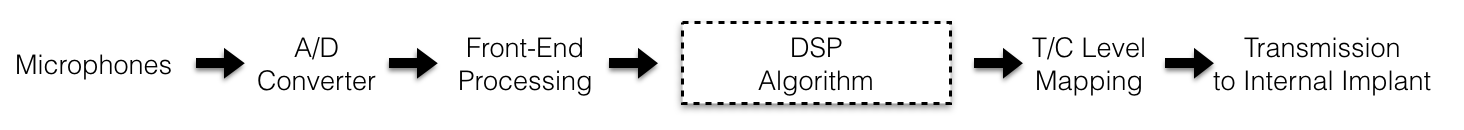
\includegraphics[width=1.0\textwidth]{CI_Signal_FlowTEMP}   
    \caption{Signal Flow in CI}
\end{figure}

In this document, the output of the DSP stage will be a strictly positive signal used to modulate a constant bipolar pulse train.

Returning to our discussion of sum-of-products models, each strictly positive signal will be composed of an envelope and carrier:

FIGURE
[DSP carrier * envelope] * pulse train = ~~~

In general we can think of the envelope as encoding the place information while the carrier encodes the temporal information

\subsection{ACE}

The simplest of the considered strategies is the Advanced Combination Encoder (ACE).  ACE has become a clinical standard for CI processing and is used in a vast number of users.  ACE is Cochlear Ltd's instance of the auditory community's generalized category of $N$-of-$M$ strategies.  In these strategies the magnitudes of the $L$ STFT envelopes are first extracted using the STFT extraction method.  These envelopes are then combined into $M$ channels corresponding uniquely to electrodes.  During each processing frame a subset $N$-of-$M$ channel envelopes is selected for stimulation on the internal implant.

$L$ - number of envelopes per frame

$M$ - number of electrode channels

$N$ - number of electrodes stimulated per frame

$$L \geq M \geq N$$

\begin{figure}[!ht]
  \centering
    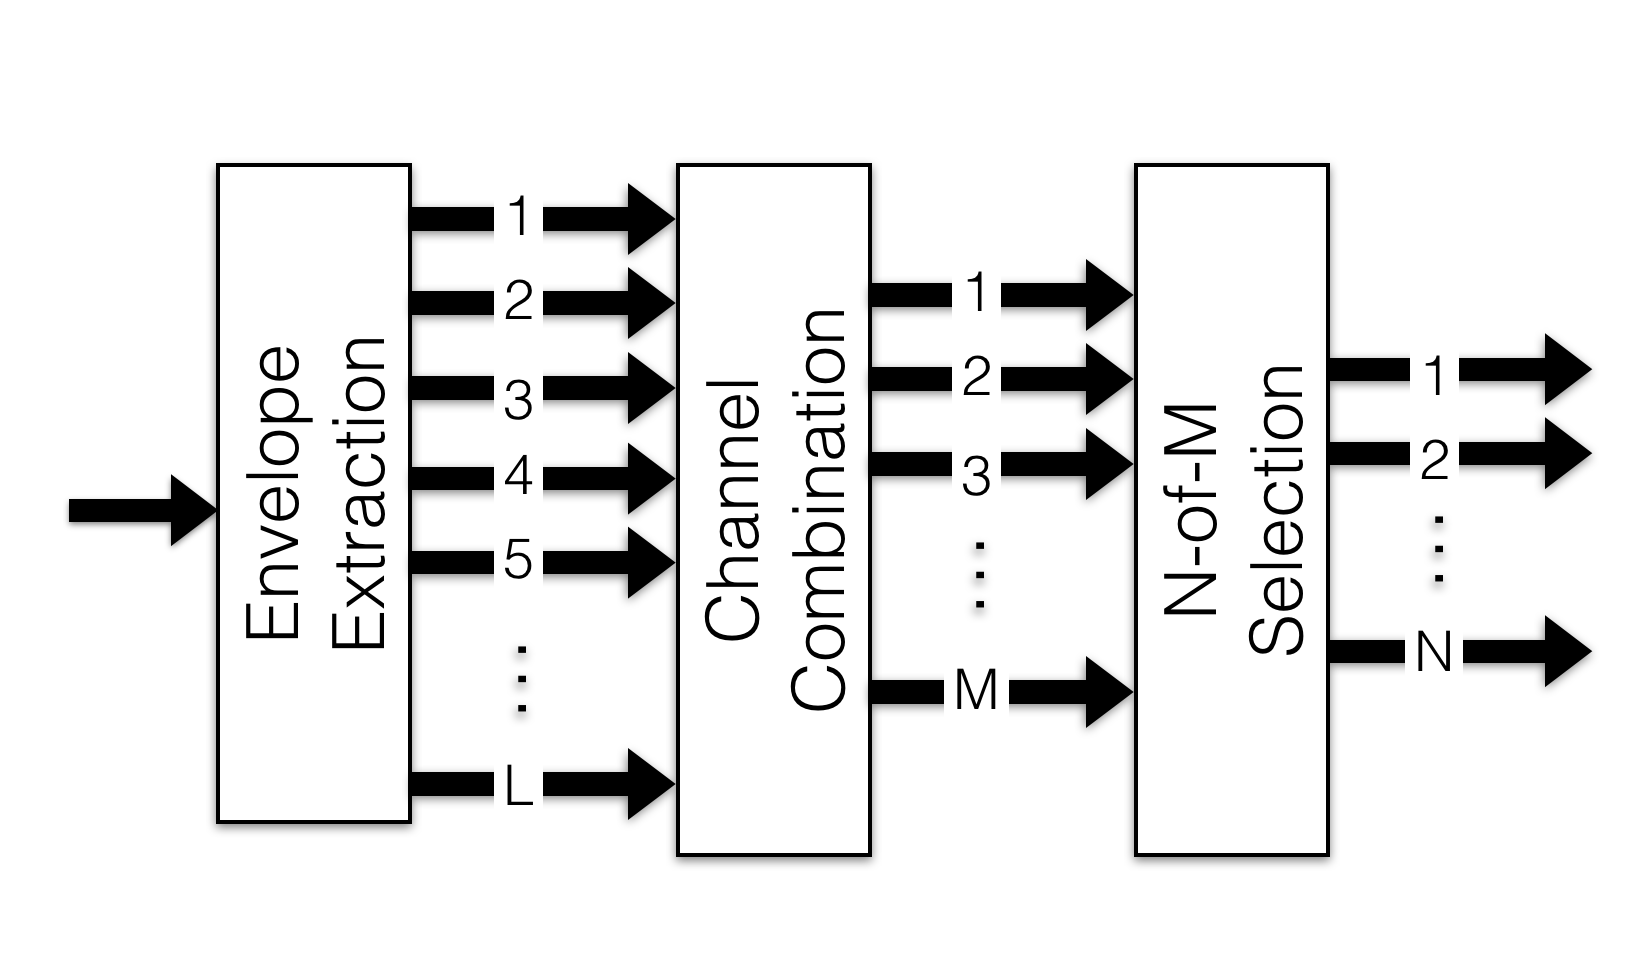
\includegraphics[width=0.5\textwidth]{ACE_flow_diagram_explicitTEMP}   
    \caption{ACE Flow Diagram}
\end{figure}

While ACE does a sufficient job for many CI users in speech recognition tasks, a large gap remains between NH and CI in pitch discrimination.  One important factor is that ACE uses place cues as the primary source of encoding a sound's characteristics.

ACE does, however, provide limited temporal modulations via beat frequencies.  This is a unique case of the filter bandwidth tradeoff in which wider bandwidth is desired to intentionally capture multiple harmonics in a band.  By doing this a beat-frequency will be induced at a rate of the difference between the two harmonic frequencies, i.e. $F_0$.  Typically these modulations are not full depth [ref?] and the depth is a function of filter rolloff, pitch and filter center frequency.  Modulations are usually limited to under ~250Hz [ref?]

The following figure is simply a condensed version of the previous flow diagram.  This condensed notation will be carried through to the other strategies analyzed.

\begin{figure}[!ht]
  \centering
    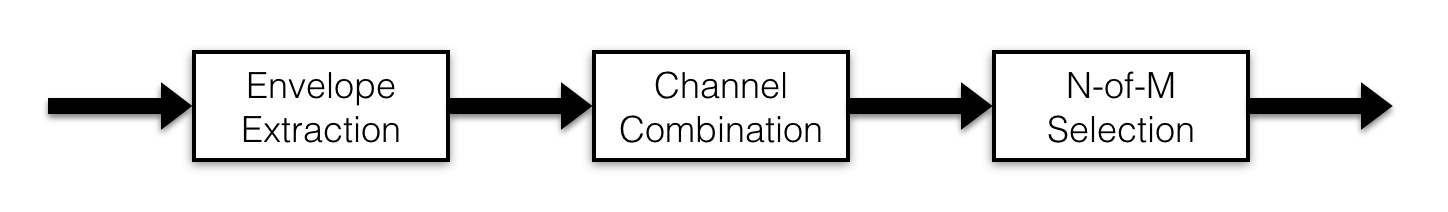
\includegraphics[width=1\textwidth]{ACE_flow_diagramTEMP}   
    \caption{condensed ACE Flow Diagram}
\end{figure}

\subsection{F0mod}

To get at the problem of pitch discrimination, (Laneau et al 2006) developed a new research strategy, F0mod.  F0mod provides the same processing as ACE with one important change, explicit carrier modulation.  It achieves this by adding a pitch estimator into the processing.

Once a fundamental frequency ($F_0$) is acquired, all output envelopes are modulated by a raised sinusoid at a rate of $F_0$.  

($F_0$ is used because high modulation rates (typically above 300Hz) are not noticeable with a CI)

This raised sinusoid is constant modulation depth, (full dynamic range), and same across channels, (phase aligned).  *maybe show a figure?  The details of modulator type are discussed later in section ?.?.  The important point here is that modulations are applied at a rate of $F_0$ and full depth.

\begin{figure}[!ht]
  \centering
    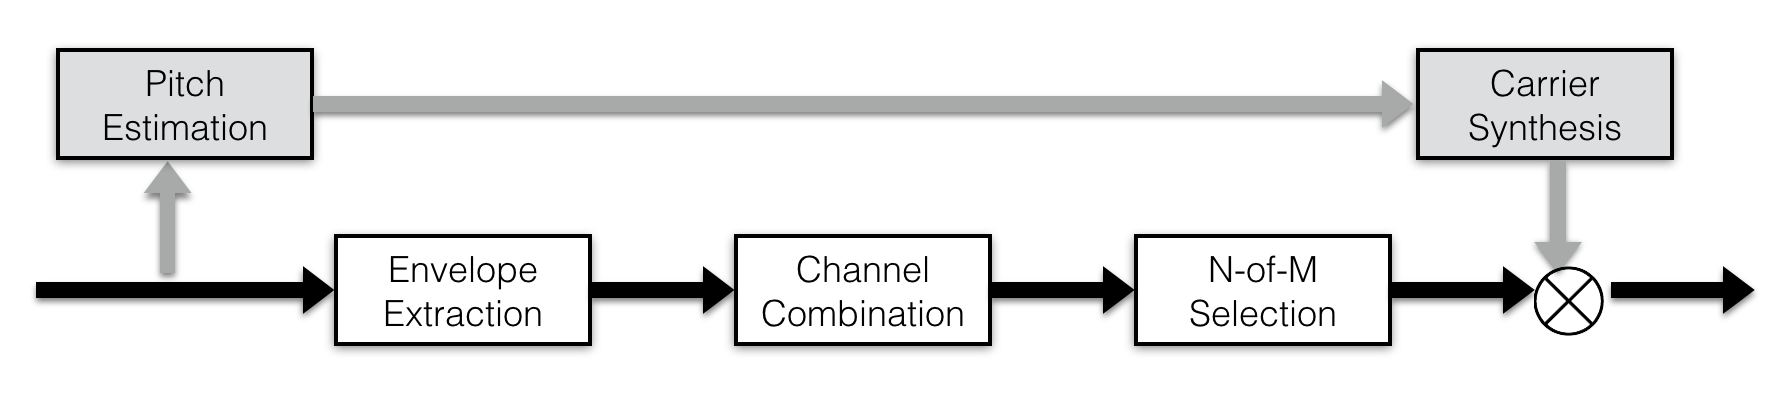
\includegraphics[width=1\textwidth]{F0mod_flow_diagramTEMP}   
    \caption{F0mod Flow Diagram}
\end{figure}

F0mod has shown promising results in acute tests for pitch discrimination.  It has also inspired other processing strategies such as eTone, which uses a more sophisticated harmonic sieve pitch estimator as well as soft decisions to overcome the problem of encoding both harmonic and inharmonic sounds as well as those that fall somewhere in between.

\subsection{HSSE}

Looking for a novel approach to improved pitch perception and more broadly music perception, (Li, Atlas, Nie) came up with Harmonic Single Sideband Encoder (HSSE).  HSSE uses coherent demodulation to extract $H$ harmonic envelopes.  These harmonic envelopes are then combined into channels based on the harmonic index and $F_0$.  Just as in F0mod a subset is selected for stimulation and then these envelopes are combined with carrier modulators.

$H$ - number of harmonic envelopes
$$H, M \geq N$$

\begin{figure}[!ht]
  \centering
    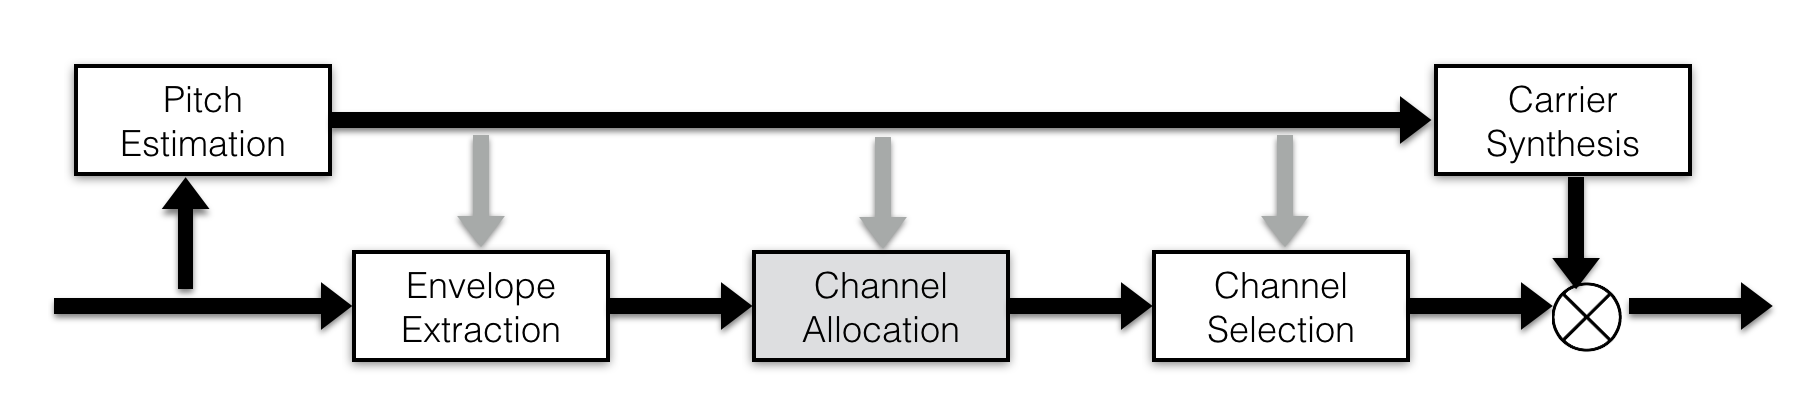
\includegraphics[width=1\textwidth]{HSSE_flow_diagramTEMP}   
    \caption{HSSE Flow Diagram}
\end{figure}

Sparing details which will soon be investigated deeper, the differences between F0mod and HSSE can be summarized quite simply;  Every stage of typical ACE processing is now done coherently using $F_0$ information.

It should be noted that it is not necessarily true that $H \geq M$.  In the case that no envelopes are allocated to a channel we may simply rule out that channel during the selection stage.

\subsection{Other Strategies}

any hybrid considerations?  maybe hint at hsse ace hybrid

talk about unmentioned methods (AB, MedEl)

\subsection{Summary}

The considered strategies can be described by five general processing blocks: Pitch Estimation, Envelope Extraction, Channel Combination, Channel Selection and Carrier Synthesis.  We will now go into detail of each of these blocks, evaluating key considerations and differences.

\section{Pitch Estimation}

Fundamental Frequency Modulation is a key prospect in temporal encoding, shared by F0mod and HSSE, but not ACE.  In both HSSE and F0mod an autocorrelation followed by peak finding is implemented.

In this method...

There are various ways to estimate pitch with trade-offs for each.  We are going to assume the pitch estimator is the same when analyzing F0mod and HSSE.


 [people] in [ref] 

talk about F0 estimator and alternatives...

    our (shared) technique
    e-tone? harmonic sieve, etc.
    latency, accuracy, octave errors and range restrictions,
    quantization

\section{Coherent Angle Encoding}

As mentioned earlier, envelope extraction results in a real nonnegative signal.  This envelope may then be modulated by a real nonnegative carrier signal.  We take a short aside to consider a method that instead generates a bandpass signal and achieves the nonnegative characteristic required for CI processing by halfwave rectifying.

In polar form, coherent envelopes are composed of both magnitude and angle components, unlike incoherent envelopes which contain only magnitude information.  [ref?] actually makes the point that decomposing a signal into magnitude and angle is not appropriate because this decomposition takes a narrowband signal and separates it into two band-unlimited components.

\subsection{Two Methods}

Let us assume for now that our carrier is a rectified sinusoid and consider a signal where our $k$th harmonic is of the form

\begin{align}
x_k[n] = A_k[n]cos(2\pi kF_0n + \phi_k[n])
\end{align}

where $A[n]$ represents a real nonnegative amplitude.  We may assume $F_0[n] = F_0$ is constant without loss of generality so long as $F_0[n]$ is roughly constant within each processing frame.

Computing a coherent harmonic envelope would result in

\begin{align}
m_{k,harmonic}[n] = A_k[n]e^{j\phi_k[n]}
\end{align}

Let us define $Rect\{y_k[n]\}$ as the rectified carrier-modulator signal which is our end goal.  One method of acquiring $y_k[n]$ is

\begin{align}
\label{eq:realVSmag1}
y_k^1[n] =& \vert m_{k,harmonic}[n] \vert cos(2\pi F_0 n) \\
=& A_k[n] cos(2\pi F_0 n) \nonumber
\end{align}

Alternatively, as proposed in [xing hsse]

\begin{align}
y_k^2[n] =& Re\{ 2m_{k,harmonic}[n] e^{j2\pi F_0 n} \}  \\
=& Re\{ 2A_k[n]e^{j(2\pi F_0 n + \phi_k[n])} \} \nonumber \\
=& A_k[n]cos(2\pi F_0 n + \phi_k[n]) \nonumber
\end{align}

It is clear that the difference between $y_k^1[n]$ and $y_k^2[n]$ is simply the extra term, $\phi_k[n]$.  What this means may be best shown by example.

In figure \ref{fig:real_vs_magnitude_example} we see that when taking the magnitude, we force symmetry about $0$.  We see that the green much better represents the blue than the red does by preserving the spectral asymmetries that manifest themselves in the angle, not magnitude.  It is unnatural and certainly won't happen in real world scenarios that a subband signal will be symmetric about the downshift frequency, however magnitude only methods force this to be true.

\begin{figure}[!ht]
  \centering
    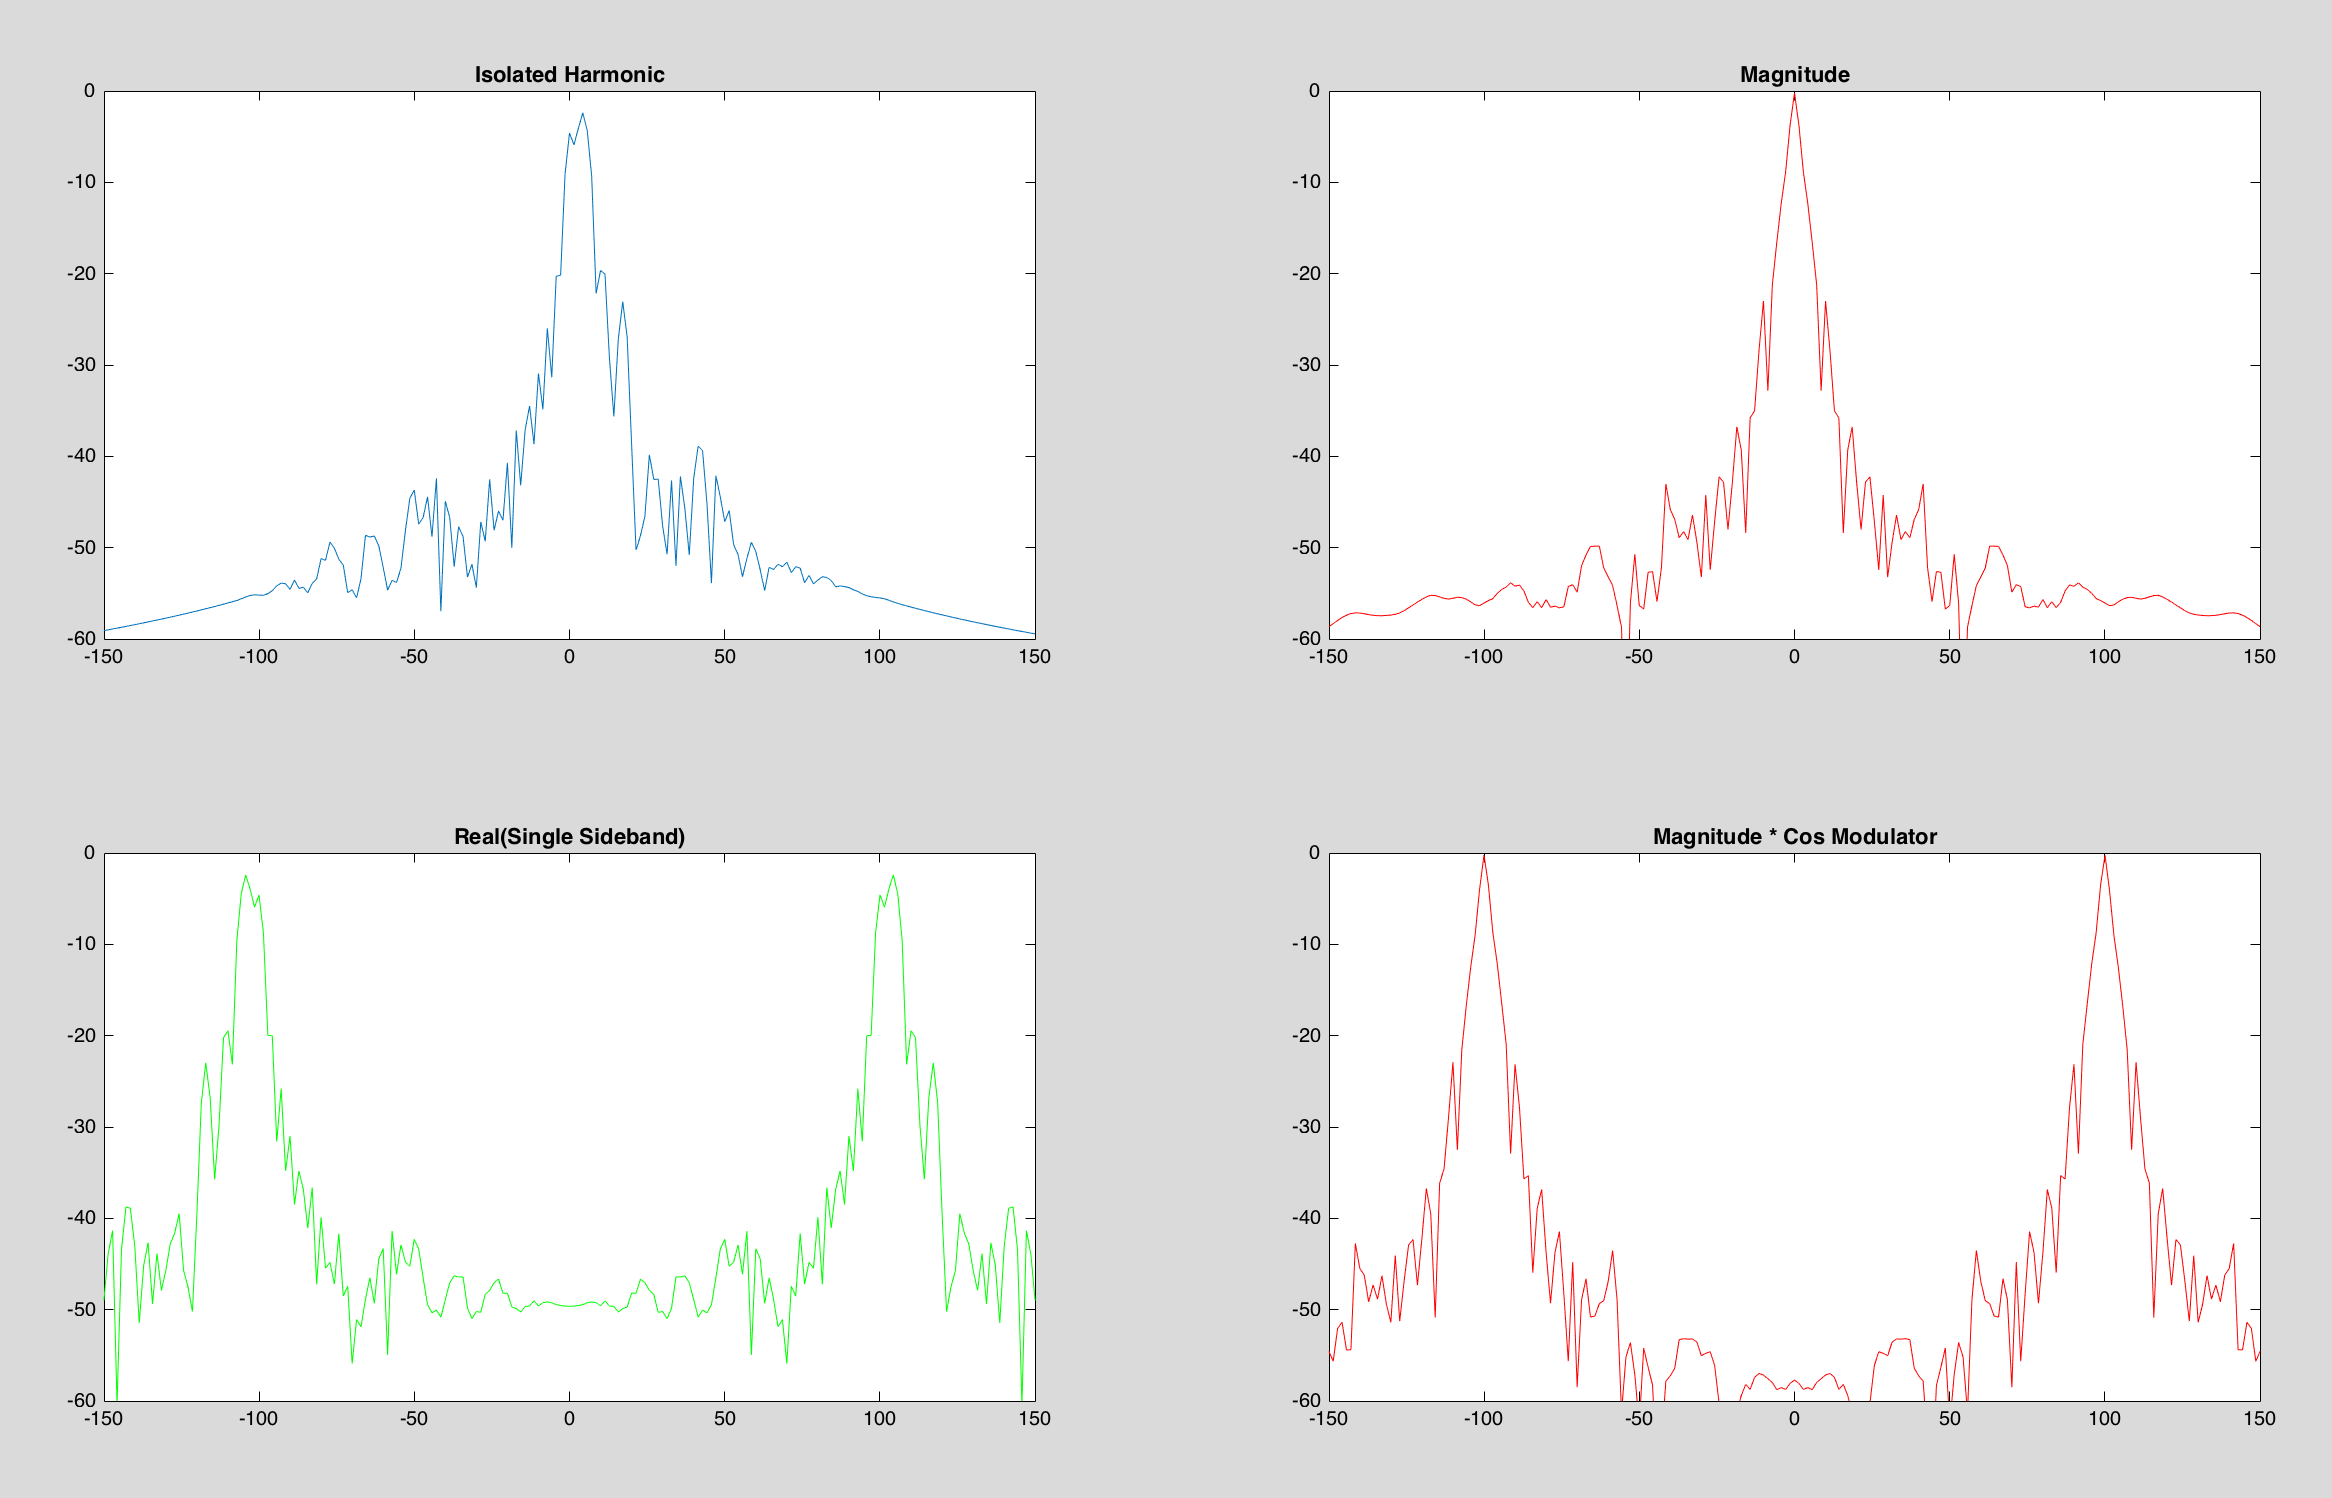
\includegraphics[width=1\textwidth]{real_vs_magnitude_example}   
    \caption{Cello Example}
    \label{fig:real_vs_magnitude_example}
\end{figure}

\subsection{Appropriate Scaling}

Despite better representing the signal, there is still an issue with $y_k^2[n]$.  The correct method is actually

\begin{align}
\label{eq:realVSmag3}
y_k^3[n] =& Re\{ 2 \vert m_{k,harmonic}[n]  \vert e^{j \frac{1}{k} unwrap(\phi_k[n])} e^{j2\pi F_0 n} \}  \\
=& A_k[n]cos\Big(2\pi F_0 n + \frac{1}{k}unwrap(\phi_k[n])\Big) \nonumber
\end{align}


Why do we need the $\frac{1}{k}$ term?  Let's consider an example where our true pitch estimate is actually $F_{0,ground truth} = F_0 + F_{err}$.  So,

\begin{align}
x_k[n] = A_k[n]cos\Big(2\pi k(F_0 + F_{err})n + \phi_k[n]\Big)
\end{align}

In this case

\begin{align}
y_k^2[n] =& A_k[n]cos\Big(2\pi (F_0 + kF_{err})n + \frac{1}{k}unwrap(\phi_k[n])\Big) \\
y_k^3[n] =& A_k[n]cos\Big(2\pi (F_0 + F_{err})n + \frac{1}{k}unwrap(\phi_k[n])\Big)
\end{align}

Essentially the term $\phi_k[n]$ may be thought of as the deviation from $kF_0$.  If we downshift the signal such that $kF_0$ is scaled to $F_0$ then it is appropriate that we scale $\phi_k[n]$ similarly.

\subsection{Efficacy}

Let us now consider the efficacy of \ref{eq:realVSmag1} versus  \ref{eq:realVSmag3}.

One hypothesis is that $\phi_k[n]$ may encode the noise-like characteristics of a signal, in which case it would remain constant for a pure sinusoid and fluctuate randomly for noise.  Put to test, the harmonic phase preservation did little to affect the signal and this was confirmed by testing varying filter bandwidths as well.  In comparison of a toy experiment, the choice of filter bandwidth dominated noise-like qualities, with wider bandwidth capturing more of the variations.

Since the term $\phi_k[n]$ does not distinguish noise-like signals from narrowband sinusoidal signals, it is only really preserving phase alignment.  But this begs the question, what does it mean to preserve the phase of a harmonic when downshifted to $F_0$?  It is questionable as to whether this even has any logical meaning.

% It means every k'th peak will be lined up with the downshifted peak, that being said that probably doesn't mean a whole lot in terms of important information
% perhaps show a figure of this?

Furthermore, it has been suggested in [REF F0mod and kaibao??] that phase alignment is important for pitch perception in CIs.  By using a magnitude-only method we guarantee alignment across channels.

Is an example necessary? Noise vs Saw example...
used "shh" vs "saw" test.  at least when listening to the simulations, the processing essentially sounds like narrowband resonant filters.  The noise-like sounds are completely dominated by the filter bandwidth and the phase-information is not noticeable at all.

Having considered this option as not a path worth further investigating, for the rest of this document we will consider envelope and carrier separately with each being a real nonnegative signal at the final output.

\section{NOTE}

mixture %

considerations:
F0 range
F0 error
Harmonic Index
F0 error mean/variance

downshift freq
BW (as function of F0?)


\section{Envelope Extraction}

As previously mentioned only envelope information is used in CI strategies.  In ACE and F0mod we use the STFT method \ref{eq:envelope_STFT}.  In HSSE we use the magnitude of the harmonic method which may be derived from \ref{eq:harmonic-to-stft} as 

\begin{align}
\label{eq:envelope_general}
m_k[n] = \frac{1}{Lw[0]} \vert X_L[n, \lambda[n]k) \vert
\end{align}

keeping in mind that this is an approximation under the assumption that $F_0[n]$ remains roughly constant over any window of time $n$ to $n + L - 1$.  $L$ denotes FFT order.

We may generalize all three methods to \ref{eq:envelope_general} by stating $\lambda[n] = 1$ for the case of ACE/F0mod.

Despite none of these methods implementing a Hilbert envelope it is useful to also consider \ref{eq:hilbert_envelope} for the potential benefits of nonuniform filter bandwidths.

We are left with two design components: downshift frequency and lowpass filter.

\subsection{limbo}

Let's consider an example?

switched-capacitor filterbanks consisted of only ~20 filters [swanson thesis] must have been non-uniform...



``From the continuum of possible frequencies, only those which coincide with the basis will project onto a single basis vector; all other frequencies will exhibit non zero projections on the entire basis set. This is often referred to as spectral leakage and is the result of processing finite-duration records.''

\subsection{Downshift Frequency}


For STFT envelopes, the downshift frequencies are fixed.  For HSSE the downshift frequencies are a function of $F_0[n]$.  Let us now consider the benefits of using $F_0[n]$.

% \ref{eq:STFTasFilter}

\begin{align}
\widehat{x}[n] =& a_0[n] e^{j2\pi \frac{F_0}{F_s} n} + a_1[n] e^{j2\pi \frac{2F_0}{F_s} n} \\
m_1[n] =& | \widehat{x}[n] e^{-j2\pi \frac{F_{DS}}{F_s} n} * w[-n] | \\
=& | \Big[ a_0[n] e^{-j2\pi \frac{F_0 - F_{DS}}{F_s} n} + a_1[n] e^{-j2\pi \frac{2F_0 - F_{DS}}{F_s} n} \Big] * w[-n] | \\
\end{align}

...ungh I'm doing a terrible job at this, the goal is to say that the downshift frequency determines the ratio of energy of harmonics.  If we downshift at exactly $F_0$ then we have maximum ratio of $x_0$ to other harmonics, relating to $|W[F_{after-downshift}]|$ for each harmonic.

The optimization of the magnitude ratio is determined by the downshift frequency, whereas the degree of mixture as well as amount of frequency beating at multiples of $F_0$ is determined by filter rolloff.

Maybe add $|W[f]|$ to some equation like the following.  Maybe do it in frequency domain, and maybe figures?!

Two things to consider, magintude of each component at baseband, and magnitude of each component at $k F_0$.

\begin{align}
m_k^2[n] =& | x_k[n] e^{-j2\pi F_{DS} n} +  x_{k+1}[n] e^{-j2\pi F_{DS} n}|^2 \nonumber \\
=& | x_k[n] |^2 + | x_{k+1}[n] |^2 + x_k[n]x_{k+1}^*[n]  + x_k^*[n]x_{k+1}[n]
\end{align}



Okay, maybe I finally have it:


\begin{align}
\widehat{x}[n] =& \sum_k a_k[n] e^{j2\pi \frac{kF_0}{F_s} n} \\
m_k[n] =& | a_k[n]| \\
\tilde{m}_k^2[n] =&  | \widehat{x}[n] e^{-j2\pi \frac{F_{DS}}{F_s} n} * w[-n] |^2 \nonumber \\
=& \Big| \sum_{k'} a_{k'}[n] e^{j2\pi \frac{k'F_0 - F_{DS}}{F_s} n}* w[-n] \Big|^2 \nonumber \\
\approx& \Big| \sum_{k'} a_{k'}[n] \Big( e^{j2\pi \frac{k'F_0 - F_{DS}}{F_s} n}* w[-n] \Big) \Big|^2 \nonumber \\
=& \Big| \sum_{k'} a_{k'}[n] \Big( e^{j2\pi \frac{k'F_0 - F_{DS}}{F_s} n} W(-k'F_0 + F_{DS}) \Big) \Big|^2 \nonumber \\
=& \sum_{k'} | a_{k'}[n]|^2 |W(-k'F_0 + F_{DS})|^2 \\
+& a_k[n]a_{k-1}^*[n]W(-kF_0 + F_{DS})W^*(-(k-1)F_0 + F_{DS}) e^{j2\pi \frac{F_0}{F_s} n} \nonumber \\
+& a_k^*[n]a_{k-1}[n]W^*(-kF_0 + F_{DS})W(-(k-1)F_0 + F_{DS}) e^{-j2\pi \frac{F_0}{F_s} n}\nonumber \\
+& a_k[n]a_{k+1}^*[n]W(-kF_0 + F_{DS})W^*(-(k+1)F_0 + F_{DS})e^{-j2\pi \frac{F_0}{F_s} n} \nonumber \\
+& a_k^*[n]a_{k+1}[n]W^*(-kF_0 + F_{DS})W(-(k+1)F_0 + F_{DS})e^{j2\pi \frac{F_0}{F_s} n} \nonumber \\
+& ...
\end{align}

There will continue to be more terms at higher multiples of $F_0$.  The first thing to point out is that these terms will become more and more negligible as one or both of the terms moves away from $|W(0)|$.  The second thing is that this motivates secondary filter if we do not want modulations since we are explicitly inducing a modulation at $F_0$ with controlled modulation depth.  The eTone strategy is an example of this, using an envelope follower...

Now lets look closer at the important term (3.17)

\begin{align}
\tilde{m}_k[n] =& \Bigg[ \sum_{k'} | a_{k'}[n]|^2 |W(-k'F_0 + F_{DS})|^2 \Bigg]^\frac{1}{2} \\
SNR =& \frac{|W(-kF_0 + F_{DS})|}{\Big[ \sum_{k'} |W(-k'F_0 + F_{DS})|^2 \Big]^\frac{1}{2}}
\end{align}







Things that should be considered when making these decisions:

-beat frequencies (good for ACE, bad for other)
    harmonic isolation
-anatomy (critical bands)
-transient/noise preservation

downshift frequency could be important at low harmonics, however for high harmonics it fails due to accuracy of F0 estimate as well as the physical process.  Humans don't resolve high harmonics, why should our system?


AN IDEA:
What about using the CIS-style last stage filter to ensure we are only getting baseband information?




The human ear has much better resolution than the cochlear implant sound processor when decomposing a signal into frequency bands.  The artifacts of this can be clearly demonstrated by example.  In case1, the energy of the signal falls directly on the center frequency of an FFT bin.  In case2 the signal falls in between two bins.  In this case, neither bin represents the true energy of the signal.

We only have so many to work with in a CI.  By using knowledge about the signal we can better design our filters to circumvent this limitation.

HOWEVER:

Coherent is the Same (mathematically) as Hilbert, as ACE, as CIS except...for the downshift frequency.  This leads to a minimal (-1.6dB max) loss of gain for the desired frequency however it may lead to lower SNRs when desired frequency is further from center of filter and noise is closer to center of filter simultaneously.

downshift frequencies are quantized to same as FFT (256 frequencies spaced 30Hz apart)
doesn't matter though, gain is same... (< -1.4dB dip)
NOT TRUE!!! Roll-off is not linear in dB, so since signal is not pure tone, components will roll off at faster or slower rates

show plots as well as math :D

how much does bin alignment matter?  it's probably a function of F0, what about unvoiced signals?
filter bandwidth? F0/2, narrower to reduce noise interference


\subsection{Filter Design}

CONTINUE HERE

filter bandwidth is a tricky one.  We could have:
constant
function of
-F0
-Fcenter

From the theoretical standpoint, envelope extraction is exactly the same in ACE and F0mod.  In implementation ACE typically uses a lower order FFT.  In [laneau] the authors consider 128-point for ACE and 512-point for F0mod and both will be considered here.



        with respect to bandwidth we actually have to different things, filter bandwidth and effective information bandwidth.  The former is obvious, the later refers to what frequencies are encoded on a electrode channel.  If multiple narrowband filters are somehow combined on the same channel, they may have the same information bandwidth as one wideband filter.





Woah...come back to CIS vs ACE etc for this!

ACE currently uses modulations due to harmonic artifacts and low-order FFT.  This is horrible!  Let me explain why...it has nothing to do with the harmonic of interest and everything to do with the one harmonic below and one harmonic above the harmonic of interest.  Because this demodulation is done incoherently the modulation depths are not directly related to the harmonic of interest.  Furthermore, the cutoff is fixed and decided by parameters of the FFT and sampling rate which have nothing to do with the signal itself.  This makes the modulation even further unrelated to the signal.  (Could this also theoretically be a problem for F0mod?  Case: $F_0$ is very low and the harmonic lands right between two bins.  A small modulation could come about, ~probably not~)

An important detail to note is that of low-order-FFT induced modulations mentioned for ACE.  Laneau explicitly describes two different methods as ACE128 and ACE512 corresponding to different FFT orders.  F0mod uses ACE512 which keeps FFT bin modulations below roughly 60Hz in contrast to ACE128's 240Hz.  This sharper cutoff keeps envelope modulations out of the carrier frequency range, isolating this component and leaving the role of carrier modulation to the explicit modulator at $F_0$.

This segregation allows for easier relation to the modulation model of sounds.  Furthermore, F0mod is not prone to the modulation artifacts present in ACE128 and discussed in section 2.?.?


\subsection{Unvoiced Signals}

I really hope!!!  This is well handled by two factors.

1) automatically choose high F0 when no good estimate exists.  This allows for higher frequencies (more important and more likely to be present in unvoiced) to be acquired.

2) If filters are adaptive bandwidth, the wide-bandwidth filters will preserve more high-frequency noise-like modulations.


 - Still no concrete solution for unvoiced signals, best answer so far is to have automatic high-F0 estimate during unvoiced sections (make it more stable than if bouncing between high and low)

\subsection{Takeaway}

 - Phase Preservation doesn't matter (shh vs saw)
 
 - center frequency also doesn't matter (-1.6dB)
 
 - HSSE may be viewed as a different way of combining FFT bin magnitudes.  I would argue that we do this using F0 for low frequencies, and fixed for high.  (critical bands!!!)

\section{Channel Allocation}

\subsection{Envelope Combination}

now that we have considered phase and magnitude, this component of HSSE can essentially be considered as a different combination of FFT bin magnitudes when compared to ACE.

as mentioned above hsse takes F0 into account and avoid bin alignment issues, however, inaccuracies in F0 estimate can lead to loosing high energy harmonics with narrowband filters.  likely need to just combine unless F0 estimator can be significantly improved

This is is where the critical band concepts come into play, would this mess up speech in noise goals? probably...but what can be done if we can't get a good pitch estimate?  filtering F0 could help this a bit but it introduces further delay

updating only 9 samples of downshift per frame rather than grabbing complete complex exponential could help however once the channels are combined it shouldn't matter

\section{N-of-M Selection 1}

The key to HSSE here, is that we have isolated individual harmonics.  Harmonics are mapped to associated fixed channels due to the limitations of a fixed number of channels and fixed locations in the cochlea.  Because we have isolated individual harmonic envelopes there is no issue of signal energy falling in between channels.

\subsection{Regularizer Heuristic}

Another bonus to HSSE is that we may add a simple heuristic to maintain channel mapping stability.  For example, if F0 has not varied significantly since the previous frame, we can allocate to the same channels to avoid unnecessary switching between channels induced by vibrato or inaccuracies in pitch estimation.

\subsection{Multiple Harmonics Per Channel}
As far as having multiple harmonics in a single channel, there are a few solutions

1) Choose highest energy harmonic.

suffers from stability issues, what about gain?

2) Choose First

suffers from missing important harmonics in channel as well as misrepresenting unvoiced signals

3) Combine

How?  via sum of squares?

does a gain factor need to be applied to each channel?  how was this determined for ACE?

\subsection{Takeaway}

Low Frequencies: stability heuristic keeps from jumping channels when on edge.

High Frequencies: not really relevant if critical bands are used

- gains?  maybe just use same as ACE since this should be pretty similar
 

\section{N-of-M Selection 2}

Two general solutions

1) Adaptive (select loudest)

similar to ACE, we can choose the loudest channels.  This suffers from stability issues.  We can apply another heuristic to stabilize the decision based on consistency of signal energy and fundamental frequency

2) Fixed

stable, each option suffers from missing key harmonics to the signal

lowest channels will imply no high frequency energy, which could be bad for unvoiced signals

other relationships such as odd harmonics or prime numbered harmonics could miss harmonics critical to timbre perception.

What if we did F0mod with same channel selections as HSSE?  What would happen?

\subsection{N-of-M Selection HSSE}

Various ideas have been proposed including $N$-largest and lowest-$N$.  Fixed Greenwood bands are determined offline, corresponding each electrode with a bandwidth.  The $N$ envelopes are then mapped to electrodes by finding the greenwood bands each harmonic falls within.


\subsection{Takeaway}

 - Fixed VS MaximaSelect: this is still up in the air, Fixed is complicated by not necessarily having harmonic envelopes
 
 - for maxima select heuristics can be used to choose same if energy and F0 have not changed significantly
 


N-of-M, It is important to note that this is the same case for F0mod.  The carrier modulation is the same on each envelope and thus does not affect the selection process.
 
 


\section{Carrier Synthesis}

talk about modulator types briefly

F0mod does raised

$$c_{ch}(t) = 0.5 + 0.5cos(2\pi F_0t)$$


We consider a few...cite paper

Let's not really go into detail about this, just mention and cite some things.  Probably put this up higher in the document?

[4 wave paper]

Swanson thesis: ``A high-rate pulse train, modulated on and off at frequency F0, had a higher pitch than a train of pulses at the rate of F0. If amplitude modulation of high-rate pulse trains is to be used to convey pitch, then the shape of the modulating waveform is important: a half-wave shape is better than a square-wave (on-off) shape.''


\section{Conclusion}


% ========== Chapter 4

\chapter{HHE}
come up with a better name!!!

MOTIVATION

\subsection{HSSE vs F0mod Differences}

harmonics are resolved

 - how do we deal with should-be-unresolved harmonics?

channel combination

 - further considerations are needed

 - what does sum of squares mean? is it constant energy within the channel?  does it cause a gain or just average the channels?  look further into the gain component to ACE
    it's just a <1 gain for multiple bins in one channel

 - can harmonics be combined? (higher harmonics) what does it mean to combine channel phase information?

channel selection

 - further considerations are needed

 - What if we did F0mod with same channel selections as HSSE?  What would happen?

\section{HSSE vs F0mod More Differences}

recitified modulator (likely not too important)

also, pitch tilts

how can all of this be applied to soft decisions?

how can this all be done in real-time?

how are we accounting for non-linearities: AGC and sensitivity




\section{Alternative Coherent Envelope Calculation using FFT bins}

This could all be achieved by zero padding, but not as efficiently?

\begin{align}
\beta = \frac{F_0}{F_s}N - \Big\lfloor \frac{F_0}{F_s}N \Big\rfloor \\
0 \leq \beta < 1 \nonumber \\
Z[k] = X[k + \beta] = X[k] * \delta[k + \beta] \nonumber
\end{align}

We can design a filter:

\begin{align}
h_{\beta}[k] =& \delta[k + \beta], \qquad 0 \leq k < N  \nonumber \\
=& IFFT\{e^{j\frac{2\pi}{N} \beta n} \}, \qquad 0 \leq n < N \nonumber \\
=& \frac{1}{N} \sum_{n=0}^{N-1} e^{j\frac{2\pi}{N}(k + \beta)n}
\end{align}

maybe be specific about circular convolution, non-infinite bounds?

\begin{align}
Z[k] =& X[k] \circledast h_\beta[k] \nonumber \\
% =& \sum_{n=-\frac{N}{2}}^{\frac{N}{2} - 1} X[((n))_N]h_\beta[k - n] \\
% =& \sum_{n=-\frac{N}{2}}^{\frac{N}{2} - 1} X[((k - n))_N]h_\beta[n] \nonumber \\
% \approx& \sum_{n=-l}^{l} X[((k - n))_N]h_\beta[n] \nonumber
\approx& X[k] \circledast h_\beta[k]w[k]
\end{align}

We have an approximation where $w[k]$ is a window and $w[k] = 0, |k| > l$.  We can then compute an approximate shift using $2l + 1$ complex multiplies and additions.  The nice thing about this is that as $|k|$ increases $h_\beta[k] \rightarrow 0$ very rapidly , so we only need a very low number $l$ to approximate with good accuracy.






Incredibly frustrating...but do we even need this?  What about just choosing the nearest FFT bin.

Another consideration: 

\section{Critical Bands}

talk about filter design in F0mod and HSSE and why non-uniform is better

\subsection{HSSE vs ACE vs Human Ear}

In this subsection I will discuss the general differences in critical bandwidth:

1) how HSSE is too fine of a resolution
note: HSSE originaly had BW = F0/2, however hard to implement and still not like ear

2) how ACE is overall a poorer resolution

What about doing a hybrid?  This would further justify alternative HSUM in it's improved efficiency!  If summing together anyway, does it matter if harmonic envelopes are used or incoherent envelopes are used?

How about specifying the bandwidth at each electrode as apposed to the frequency boundaries

Bro, you need to look into Xing's method with multiple harmonics modulated at multiples of F0...
%curK in HSSE_all_harmonics_halfF0_8_dynamic_channel_Xing.m


\subsection{Resolution Simulated by Adaptive Envelopes}

The human ear has orders of magnitude more filters than ACE, (roughly 1500/22 I think).

HSSE could simulate this higher resolution by choosing different filter center frequencies based on the input signal

\subsection{Channel Selection Analysis}

ACE is like HSSE but for fixed FoI's.  We extract an envelope at the FoI and then transmit it to the associated electrode.

1) this goes back to what are the implications of ACE512 vs ACE128 vs coherent-envelope if we are summing anyway

2) can HSSE be reanalyzed in these terms to better justify wide-bandwidth filters for high frequencies?

Could channel selection concepts in HSSE be important?  Reflect on this in hindsight to recent discoveries.  By this I mean using memory to not switch channels excessively and other decisions that were brought into account.

\section{Other Important Components}

Most everything so far has assumed the signal has an $F_0$, what if it doesn't?  What if it is well outside the boundaries of $F_0$?  What about polyphonic music?  What about SNRs below what is needed for accurate $F_0$ estimation.  What other flaws do these strategies have?  Mention eTone and other possible solutions, or why we justify not considering these problems.

\section{Algorithm}

1) Filter Center Frequency
2) Filter BW
3) Effective Channel Information BW

\section{Freedom details}

% ========== Chapter 5

\chapter{Subject Tests}
initial results are...



 it was important not to change other
12 HWR strategy take-home study 224
aspects of the strategy, in particular, stimulation rate. It would not be a fair comparison to trial HWR at 1800 pps against ACE at 900 pps, as the increased stimulation rate in itself could affect performance. A higher rate could potentially represent amplitude modulation cues more faithfully (McKay et al. 1994). Conversely, there is evidence that sensitivity to temporal modulation is worse at higher rates (Galvin and Fu 2005).
[swanson thesis]

    \subsection{simulated real-time}
    
    \subsection{mandarin tones pitch tilt}
    
    \subsection{freedom processor}
        speech recognition...
        timbre recognition...
        other...


% ========== Chapter ??
 
\chapter{Less Theoretical Stuff}

About this chappy

\section{Engineering Decisions for Real-time}

1) 8 harmonics
this assumes we are dealing with musical instruments, speech is going to have characteristics well above the 8th harmonic.  A hope is that with inharmonic signals the estimate will automatically bounce to max($F_0$ estimate) which will thus hit the highest frequencies.  This also goes back to the hybrid idea


2) $F_0$ estimation downsampling details, ooOOooo, so impressive!

\section{$F_0$ tilt, exageration}

mention the point that this was already done in Xing's paper, albeit $F_0/2$ without affine shift is more more likely to hit boundaries 

\section{assembly implementation}

maybe show flow diagram or talk about 128-pt fft limitations



% ========== Chapter 6

\chapter{Conclusion}

\section{Summary}

\section{Future Work}



%
% ==========   Bibliography
%
\nocite{*}   % include everything in the uwthesis.bib file
\bibliographystyle{plain}
\bibliography{ganter_thesis}
%
% ==========   Appendices
%
\appendix
\raggedbottom\sloppy
 
% ========== Appendix A
 
\chapter{Where to find the files}
 
The uwthesis class file, {\tt uwthesis.cls}, contains the parameter settings,
macro definitions, and other \TeX nical commands which
allow \LaTeX\ to format a thesis.  
The source to
the document you are reading, {\tt uwthesis.tex},
contains many formatting examples
which you may find useful.
The bibliography database, {\tt uwthesis.bib}, contains instructions
to BibTeX to create and format the bibliography.
You can find the latest of these files on:

\begin{itemize}
\item My page.
\begin{description}
\item[] \verb%http://staff.washington.edu/fox/tex/uwthesis.html%
\end{description}

\item CTAN
\begin{description}
\item[]  \verb%http://tug.ctan.org/tex-archive/macros/latex/contrib/uwthesis/%
\item[]  (not always as up-to-date as my site)
\end{description}

\end{itemize}

\vita{Jim Fox is a Software Engineer with UW Information Technology at the University of Washington.
His duties do not include maintaining this package.  That is rather
an avocation which he enjoys as time and circumstance allow.

He welcomes your comments to {\tt fox@uw.edu}.
}

\end{document}
